% arara: xelatex
% arara: xelatex
% arara: xelatex

% options:
% thesis=B bachelor's thesis
% thesis=M master's thesis
% czech thesis in Czech language
% english thesis in English language
% hidelinks remove colour boxes around hyperlinks

\documentclass[thesis=B,english]{FITthesis}[2019/12/23]

\usepackage[utf8]{inputenc}
\usepackage{dirtree}
\usepackage{graphicx}
\usepackage{amsmath}
\usepackage{algorithm}
\usepackage{algorithmic}
\usepackage{listings}
\usepackage[export]{adjustbox}





\newcommand{\tg}{\mathop{\mathrm{tg}}} %cesky tangens
\newcommand{\cotg}{\mathop{\mathrm{cotg}}} %cesky cotangens

\department{Katedra softwarového inženýrství}
\title{Visual Analysis of Plans for Multi-Agent Path Finding with Continuous Time (MAPF-R)}
\authorGN{Evgenii}
\authorFN{Abdalov}
\authorWithDegrees{Evgenii Abdalov} 
\author{Evgenii Abdalov} 
\supervisor{doc. RNDr. Pavel Surynek, Ph.D.}
\acknowledgements
{
  I would like to give thanks to my supervisor doc. RNDr. Pavel Surynek, Ph.D., who was leading the path to my deeper understanding of Multi-Agent Path Finding problems with his advice and knowledge.
}
\abstractCS
{
 Tato práce je věnována vytvoření vizualizačního nástroje za účelem zprostředkování vizuální analýzy problému Multi-agentniho hledani cest v nepřetržitem čase (MAPF-R). Popisuje problém MAPF-R, poté pokračuje popisem vývoje vizualizačního nástroje a ekonomickým hodnocením jeho potenciálu využití v logistické oblasti.	
}
\abstractEN
{
  This thesis is dedicated to creation of visualization tool in order to convey visual analysis of Multi Agent Path Finding with Continuous Time(MAPF-R) problem. It describes MAPF-R problem, then it continues with description of development of visualization tool and economic evaluation of its usage potential in logistics domain.  	
}
\placeForDeclarationOfAuthenticity{V~Praze}
\declarationOfAuthenticityOption{4}
\keywordsCS{Závěrečná práce, MAPF-R problem, vizualizace}
\keywordsEN{Thesis, MAPF-R problem, visualization}
\website{https://gitlab.fit.cvut.cz/abdalevg/bp_evgenii_abdalov} 


\begin{document}

\begin{introduction}
In modern technological and economical environment the importance of data has increased dramatically. As a matter of fact, data-driven desicion making has a lead role in succesfull management techniques. Nevertheless, in order to extract genuine value from your data, the one must process data correctly. Dealing with vast amount of data has a potential to increase probability of making a miscalculation in data processing. In such situation we could implement tools that facilitate visual analysis of data, i.e. use visual interfaces to process data.

Among various algorithmic problems there is a certain class of problems, that requires proper visual analysis in order to be solved correctly - those are problems on graphs. Graph is an abstraction, that models interconnections between set of objects. It is a collection of vertices and edges, that are defined by pairs of vertices. One of the most common type of problems that are solved on graphs is space-orientated problems, where vertex is an abstraction for a location(cities,rooms, airports) and an edge is an abstraction for a route between them. The problem is commonly stated, that we need to find the shortest path from a location A to a location B. Let's make an assumption that there is only one agent, that travels on graph. In this case, in order to succesfully find a path we need to take into account only restrictions that are put by space-graph. However, if we add more agents, that are travelling on graph, we should take other agents movements as a restrictions that must be considered while finding the solution. This kind of problems is called Multi-Agent Path Finding problem. Multi-Agent Pathfinding(MAPF) problem deals with finding paths for multiple agents, so they can avoid collisions with each other and reach their target destination. The solution to MAPF problem is as complex as amount of agents involved, which leads to the necessity of using visual analysis of the solution. Thus, there is a motivation to design a visualiation tool. Visualization of MAPF problem is crucial for further analysis of the solution, finding its redundancies and detecting ways to make it more effective.
   
The main goal of this thesis is to design and develop a visualization tool for multi-agent pathfinding problem with continuous time that enables its visual analysis. In interest of achieving this goal, following tasks must be accomplished. Initially,we should study relevant literature on MAPF-R problem and identify aspects deserving visualization. Secondly,
we will design and implement visualization tool of MAPF-R plans. After that, provide documentation of both the user part and the program so that future upgrades are possible.
Finally, analyze economic potential of the visualization tool in logistic domains where MAPF-R is used as an underlying concept for navigating robotic manipulators.

\end{introduction}

\chapter{Understanding of MAPF-R problem and its visual analysis}

In this chapter we will determine theoretical basis of MAPF-R problem,
secondly we will characterize what visual analysis is, its main functions and tools,
and indicate essential aspects of MAPF-R problem that have to be visualized.


\section{Motivation}

Modern economical and technological environment has a tendency to increase the level of automation involved in production process. Although automation is advantageous for production effectivness and speed, it still needs to be controlled and monitored by a human operator. Therefore increased usage of robotic manipulators and AI-based desicion making routine requires to be provided with adequate \verb|visual interfaces|.

This bachelor thesis aims to provide with a visual interface for one particular problem in automation domain, which is the Multi-Agent Path Finding problem in continuous time.\ref{fig:float107} \ref{fig:float108}

\section{Multi-Agent Pathfinding problem description}

Multi-Agent Pathfinding problem deals with planning paths for multiple agents
so they can avoid collisions with each other and reach their target destinations.
The MAPF problem has a vast range of domains where it is being applied, including robot planning, autonomous vehicles, videogames, automated warehouses. 

The input of standard MAPF problem for k agents is a tuple $<G,s,t>$, where G = (V,E) is a graph, $s:[1,....,k]$ is a set of starting vertices for k agents, $t:[1,....,k]$ is a set of target vertices for k agents. Action is a function $a:V->V$, where $a(v)->v'$ suggests that if an agent is at vertex $v$, after performing action A it will be in vertex $v'$. Every agent has two types of actions: \verb|wait| and \verb|move|. \verb|Wait| means that agent stays at the current vertex, \verb|move| means that agent moves from its current vertex $v$ to an adjacent vertex $v'$. Single-agent plan is a sequence of actions $\pi = (a1,....,an)$, that leads agent $i$ from $s[i]$ to $t[i]$ after being executed. The output of standard MAPF problem is a solution $\pi = (\pi 1,...., \pi k)$, that contains k single-agent plans, where one agent has one single-agent plan.\cite{bib_1}

The majority of MAPF problems is solved on grids with discrete time, where the duration 
of every action is one time step and each agent occupies exactly one single location in every time step. All agents are considered to be of the same shape and size and have the same constant speed. It uses space-time maps to describe agent's location at a certain moment of time - $Cell(x, y, t)$, where $(x,y)$ are space coordinates on the map and $(t)$ is a timestep. 

The standard MAPF problem includes such types of conflicts as:
\begin{description}
\item[vertex conflict]  occurs if agents are planned to occupy the same vertex at the same time step.
\item [edge conflict]   occurs if agents are planned to traverse the same edge at the same time at the same time-step in the same direction.
\end{description}

The solution has addional parameters, that evaluate a MAPF solution.
\begin{description}
\item [makespan] is the number of time steps, that are required for all agents to reach their target position. For a MAPF solution $\pi = (\pi 1,...., \pi k)$, the makespan is $\|\pi i\|$, where $\pi i$ is a single-agent plan with the maximum amount of steps for agent i.
\item [sum of costs] is the sum of time steps, that are required for each agent to reach their target position, which is $\displaystyle\sum 1 \leq i \leq k\|\pi i\|$. 
\end{description}

The MAPF problem in descrete time is less applicable in real life situations, where processes occur in real time environment. The MAPF-R is Multi-Agent Pathfinding with continuous time, where agent motion is planned for a certain time interval. This time interval is a minium time considered to be safe for planned actions, which means there would be no collisions during this time interval. Similar to the standard MAPF problem, MAPF-R has as an input a workspace and agents parameters. Workspace is a 2D space, which can be represented as a graph G = (V, E), where vertices V are location, that agents can occupy, and edges E are line trajectories, which agents move along. Agents parameters are start location and target location. An output of algorithm is a MAPF-R problem solution, which is a joint plan for agents. Joint plan consists of individual plans for each agent, where the plan is a sequence of actions for agent needed to be taken so it could reach its target position. Duration of a move is translation speed times the length of the edge. In order to evaluate the MAPF-R solution such parameters as the makespan and the sum of costs are still applicable, however the definition of a plan cost differs. Instead of the number of time steps, cost of a plan is the sum of the durations of its constituent actions. 


\section{Conflict based search algorithm}

When focusing on algorithms that solve MAPF problem, the key requirement is that the solution has to be cost-optimal. Although there are several algorithms for solving MAPF-R problem, algorithm, that is considered the most efficient, is CBS, which stands for  Conflict based search algorithm.

First, CBS in discrete time should be described. As an input we have workspace and agents parameters. The path is how agent $i$ moves on space-time grid, \verb|solution| is a set of $k$ paths for the given set of $k$ agents. Generally speaking, the conflict-based search algorithm finds separate plans for each agent, then it determines conflicts between those plans and solves it by replannig whith specific constraints, that has been put on individual plans.

There is two types of \verb|constraints| in conflict-based search algorithm, which are vertex constraint and edge constraint, Vertex constraint $(a[i], v, t)$ is a configuration when agent $i$ is not allowed to occupy vertex $v$ at the time $t$. Similarly to vertex constraint, edge constraint $(a[i], v1, v2, t)$ is a configuration when agent $i$ is not allowed to start moving from vertex $v1$ to vertex $v2$ at the time-step $t$ and arriving at the time-step $t+1$. We say, that \verb|path| for agent $i$ is \verb|consistent| if it satisfies all its \verb|constraints|. The \verb|solution| is \verb|consistent| if all its \verb|paths| are \verb|consistent|. 

Two types of \verb|conflicts| are being considered in CBS: a \verb|vertex| conflict and an \verb|edge| conflict. A vertex conflict is a situation $(a[i], a[j], v, t)$, when agents $i$ and $j$ are planning to occupy vertex $v$ at the same moment of time $t$. An edge conflict is a situation $(a[i], a[j], v1, v2, t)$, when agents $i$ and $j$ are planning to swap locations $v1$ and $v2$ between time-step $t$ and time-step $t+1$. The solution to MAPF problem is considered to be \verb|valid|, in case there is no conflict between any two single-agent plannings. In spite of being consistent, solution can be invalid if this solution has paths that have conflicts with each other. \verb|Conflicts| are resolved by imposing \verb|constraints|.

CBS consists of high-level search and low-level search. The high-level search is a constraint-tree CT, which is a binary tree. Every node N includes a set of constraints(N.constraints), a solution(N.solution) and the total cost(N.cost). The root of CT has an empty set of constraints. The child node inherits parent constraints and adds to that one new for one agent. One node consists of constraints for only one agent. The solution inside the node is a set of $k$ paths, one path for each agent. These paths must be consistent with given constraints - path for agent $i$ is consistent with constraints imposed to agent $i$. The total cost is summed over all the single-agent path costs.   

As far as low-level search is concerned, any single-agent pathfinding algorithm(SIPP) can be used, for example A*. The low-level search is looking for individual paths for each agent with given set of constraints. As an input for the low-level search a set of constraints for a node N is given. As an output, low-level search returns the shortest path for agent $i$ that is consistent with imposed constraints assosiated with agent $i$ in node N. Afterwards, \verb|validation| of the node has to be processed. The \verb|validation| is conveyed by iterating through all the time-steps and matching the locations reserved by all agents. The node N is declared to be the \verb|goal| node in case there is no conflict, i.e. no two agents plan to be at the same time at the same location. On the contrary, the node N is declared to be the \verb|non-goal| node if a conflict $C = (a[i], a[j], v, t)$  between two or more agents has been found as a result of \verb|validation|.

In order to resolve a conflict $C = (a[i], a[j], v, t)$, a new constraint must be added. It is illustrated in \ref{fig:float1}. Only one agent $i$ or $j$ is allowed to occupy location $v$ at a time $t$, subsequently two options is possible - impose a constraint $(a[i], v, t)$ or a constraint $(a[j], v, t)$. We need to explore both options, as we are not aware which one is more optimal then another. Therefore, a non-goal node N is split onto two children, each one obtains a new constraint, $(a[i], v, t)$ and $(a[j], v, t)$, and inherits the set of constraints from its parent - N.constraints. Note, that low-level search may be performed only for an agent which is connected with newly added constraint, as other agents paths remain the same since no new constraints have been added for them. The high-level search treats edge conflicts in a similar manner as vertex conflicts. In case plan does not have neither vertex nor edge conflicts, the solution has been found.

\begin{algorithm}
\caption{High level of CBS}
\begin{algorithmic}[H]
\STATE {Input: MAPF instance}
\STATE {Root.constraints = \{null\}}
\STATE {Root.solution = find individual paths by the low\_level\_search()}
\STATE {Root.cost = SIC(Root.solution)}
\STATE {insert Root to OPEN}
\STATE {}
\WHILE {OPEN not empty} 
 \STATE {P $<-$ best node from OPEN}  
 \STATE {Validate the paths in P until a conflict occurs}
 \IF {has no conflict}
      \STATE {return P.solution}
 \ENDIF
 \STATE {C $<-$ first conflict $(a[i], a[j], v, t)$ in P}
 \FOR {agent a[i] in C}
 \STATE {A $<-$ new node}
 \STATE {A.constraints $<-$ P.constraints + $(a[i], v, t)$}
 \STATE {A.solution $<-$ P.solution}
 \STATE {Update A.solution by invoking $low\_level\_search(a[i])$}
 \STATE {A.cost = SIC(A.solution)}
 \IF {A.cost $<$ INF}
    \STATE {Insert A to OPEN}
 \ENDIF   
 \ENDFOR       
\ENDWHILE
\end{algorithmic}
\end{algorithm}

CCBS, conflict based search algorithm in continuous time follows CBS pattern. However,
CCBS has its differences from CBS. In order to detect conflicts, CCBS uses a geometry-aware
collision detection mechanism. In order to resolve conflicts, CCBS uses a geometry-aware unsafe-interval detection mechanism. Instead of location-time pairs, CCBS adds constraints 
over pairs of actions and time ranges. CCBS lower-level search uses a variation of SIPP, single agent pathfinding algorithm, customized to handle CCBS constraints.

In CCBS agents can have any geometric shape, different speed and acceleration and agent's actions can have any duration, a conflicts in CCBS can occur between agents traversing different edges. Conflict in CCBS is a conflict between \verb|actions|. Formally speaking, a conflict configurtion $(a[i], t[i], a[j], t[j])$ means, that if agent $i$ executes action $a[i]$ during the time period $t[i]$ and if agent $j$ executes action $a[j]$ during the time period $t[j]$, then collision will happen between agent $i$ and $j$.

In CCBS the high-level search is similar to its discrete version in CBS. It also uses CT to resolve conflicts by imposing constraints. The collision \ref{fig:float103} detection mechanism determines if node N is a goal node. In case node N is a non-goal node, it splits into two children nodes with new constraints. In order to compute new constraints, that will be added, CCBS finds for each action its \verb|unsafe| intervals. The unsafe interval of action $a[i]$ is the maximal time interval starting from $t[i]$ during which performing $a[i]$ will cause a collision with performing performing $a[j]$ at a time $t[j]$. 

In terms of low-level search, CCBS uses SIPP adopted to handle continuous time constraints.
For each location $v \in V$ SIPP finds a set of \verb|safe intervals|. A safe interval is considered to be a maximal time interval in which an agent is able to arrive or wait at location $v$ without colliding with any moving obstacles. Extending a safe interval in any direction will lead to collision, thus this safe interval is \verb|maximal|. Let's assume 
$C = (i, a[i], (t1, t2))$ is CCBS constraint for agent $i$. In this case action $a[i]$ may be \verb|wait| action or \verb|move| action. In case, $a[i]$ is a \verb|wait| action, let
$v$ be a start location and $v'$ be a target location. If the agent arrives at $v$ in time step $t \in [t1, t2)$ then we delete an action that moves agent from $v$ to $v'$ during the time period $t$ and exchange it for an action that is waiting at $v$ until $t2$, and then agent is allowed to move to $v'$. In case $a[i]$ is a \verb|wait| action, let $v$ be a location at which the agent is waiting. Then, we forbid the agent from waiting during $t \in [t1, t2)$ by splitting safe intervals accordingly - if $[0, INF)$ is considered to be solely one safe interval for location $v$, then we split it in two safe intervals $[0, t1]$ and $[t2, INF)$.\cite{bib_2}



\begin{figure}\centering
	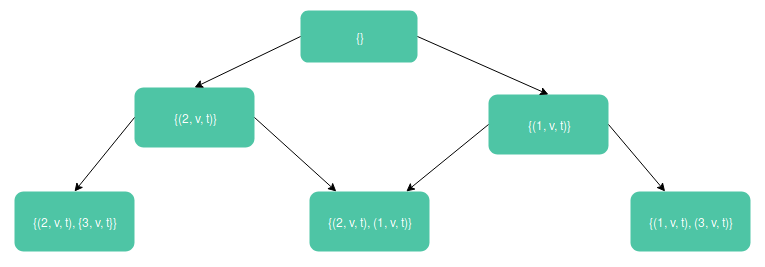
\includegraphics[scale=0.5]{binary_CT.png}
	\caption[example of CT binary tree]{example of CT binary tree}\label{fig:float1}
\end{figure}

\begin{figure}
	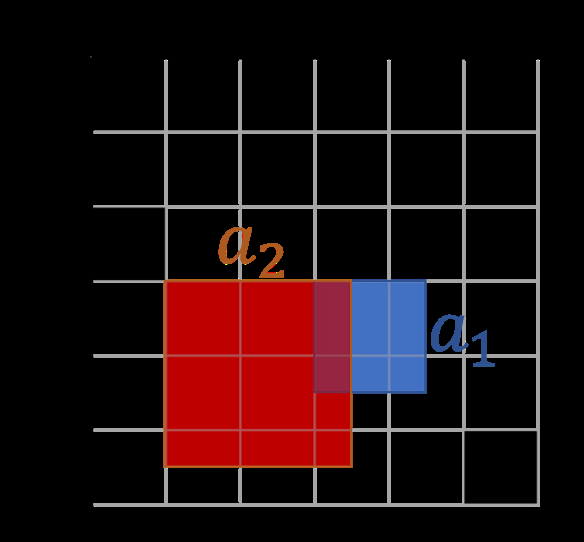
\includegraphics[scale=0.35]{collisionEvent.png}
	\caption[Example of two agents colliding]{Example of two agents colliding}\label{fig:float103}
\end{figure}


\begin{figure}\centering
	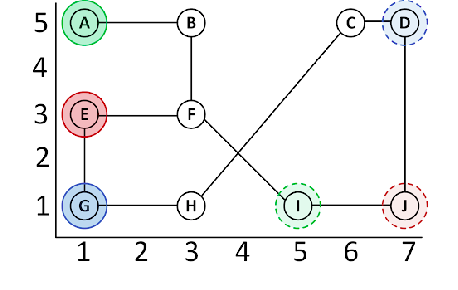
\includegraphics[scale=0.5]{MAPF-R.png}
	\caption[a. MAPF problem]{a. MAPF problem}\label{fig:float107}
\end{figure}



\begin{figure}\centering
	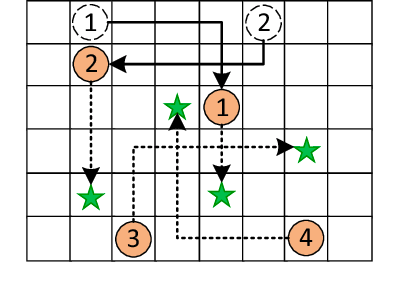
\includegraphics[scale=0.5]{MAPF-R2.png}
	\caption[b. MAPF problem]{b. MAPF problem}\label{fig:float108}
\end{figure}

\section{Visual analysis}

In this section visual analysis of MAPF-R problem will be discussed. The correct MAPF-R problem visualization is necessary as long as it allows to convey a visual analysis of the solution. Visual analysis is meant to facilitate the detection of conflicts and redundant elements in terms of output solution. As a matter of fact, in case of the MAPF-R problem containing tens to hundreds of agents it is extremely hard to determine if output solution is correct without visual representation \ref{fig:float2}.

\subsection{Visual analysis methods and tools}

\begin{figure}\centering
	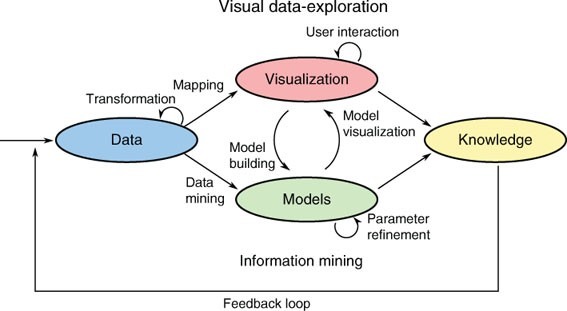
\includegraphics[scale=0.5]{model1.jpg}
	\caption[The Visual Analytics process]{The Visual Analytics process}\label{fig:float2}
\end{figure}

Visual analytics is described as the science of analytical reasoning assisted by interactive visual interfaces. Visual analysis incorporates aspects of \ref{fig:float3}
\begin{itemize}
\item visual representation
\item user interaction
\item algorithmic analysis
\end{itemize}


Those aspects are a foundation of a sufficient visual analysis tools and are closely interconnected. For instance, algorithmic analysis may function as a preprocessing step that determine specific graph layout for visual representation. 

User interaction aim to discover different aspects of the data by changing visual representation and requesting different algorithmic processing of the data. User interaction may be minimal, where data is processed automatically, or, on the contrary, data processing is fully dependent on parameters inserted by user. User interaction can be classified by such criteria as 
\begin{itemize}
	\item user intention
	\item task
	\item user action   
\end{itemize}

Those criteria are interrelated; for example, one task might be obtained by performing several actions, or several intentions might include the same task. As far as graph visualization is concerned, standard user interaction techniques might be applied, such as highlighting, brushing, linking, panning and zooming. Zooming and panning facilitate navigation in any direction and change the zoom level within the view. Highlighting is making an emphasis on interesting elements of the visual representation.

\begin{figure}
	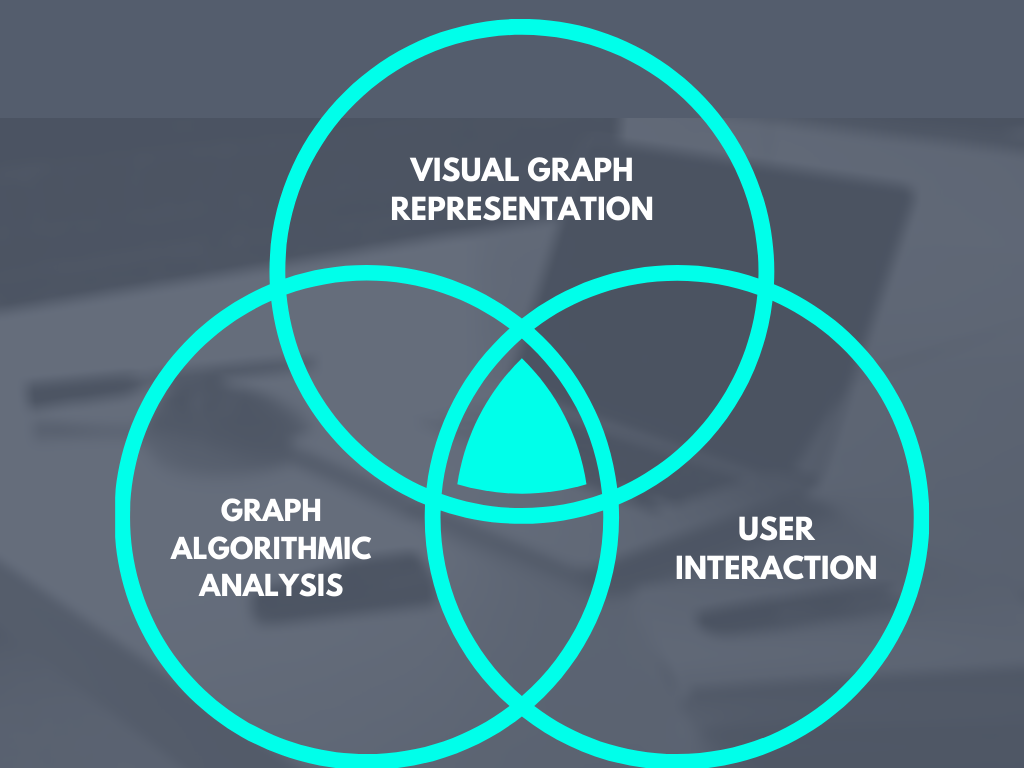
\includegraphics[scale=0.25]{visualgraphrepresentation.png}
	\caption[The main components of visual graph analysis]{The main components of visual graph analysis}\label{fig:float3}
\end{figure}

\subsubsection{Graph visual representation}

There are three main techniques for displaying general graphs: node-link based, matrix-based and hybrid. The \verb|node-link based| technique is more compatible with our needs for a visualisation tool. Node-links techniques use links between graph elements to display their relationship. The main challenge of this technique is the layout, which is the placement of the nodes, so that certain degree of graph readability is supported. The main requirements to the layout are: the nodes must not overlap, the number of edge crossing must be minimal, edge lenght should be homogeneous. Such tasks are solved by specific graph layout algorithms. There is a sub-technique, which is \verb|graphs with geographic reference |, for example transportation graph. The geographic location dictates the precise location of the nodes and possibly of the edges. Subsequently, there is no need for a graph layout algorithm in order to place nodes on the screen, although there might be problems with long edges and crossings.\cite{bib_3}

\subsection{MAPF-R problem visualization theory}

As an input data set MAPF-R visualisation tool will operate with graph charachteristics, agent parameters and its plans. The graph characteristics data set is composed of following components: 
\begin{itemize}
	\item a number of edges
	\item a number of vertices and which ones are connected with edges
	\item coordinates for each vertex within the cartesian coordinate system
\end{itemize}

The agent parameters data set includes agent shape and size parameters, its velocity and acceleration, and agent start position as well as agent target position. The agent plans data set represents agent behavior within the timeline, i.e. agent action during specific time intervals.     

Visual representation is based on data, which means that any modification in data affects the visual representation. For instance, data filtering influences which parts of the data set are going to be displayed and that could change graph modification or layout. In case of MAPF-R visualisation tool, user does not modificate or filter data set, although user could input different agent plans for the same graph, which results in different agent movement animation on the same graph layout. 


As far as visual representation is concerned, the main challenge is to establish an acceptable level of physical abstraction, i.e. determine which aspects of problem should be visualized and which could be ignored. The workspace is presented as a graph on 2D space, where nodes interconnected with edges mean that agent is physically allowed to traverse between them. The position of vertices are specified by coordinates within the cartesian coordinate system. Edge between two vertices is a line connecting two points. The exact position of edges is imperative since it has direct influence to the possibility of collision between agents. Other physical parameters of space, such as lightning, air temperature, floor level, height of ceiling, can be ignored in visualization.

As previously stated, MAPF-R problem takes into account agent physical shape and size, subsequently physical restrictions, which are implied, should be visualized properly. It will allow user to detect danger areas, where the risk of collision between agents is higher than average. Since agent's constraints are presented as a set of time intervals, agent have to move in real time according to its velocity and acceleration.

\subsubsection{Statistical analysis}

In addition to visual representation, we aim to collect statistics data as a part of data analysis. Data analysis enhances visual observation and facilitates the probability of making an analytical discovery. The statistics data indicates algorithm perfomance and effectivness. In case of MAPF-R problem visualization tool, we will collect data about overall time duration of the solution as well as time duration for individual agents to reach its target destination from starting point. Furthermore, we aim to collect data of how much time agent moves and how much time agent waits, using this data we could estimate moving/waiting ratio for each agent. 

Using \verb|visualisation analysis| in combination with \verb|data analysis|, it is possible to perform a comparison analysis of several MAPF-R problem solutions. Based on this analysis it is feasable to find out which algorithm solves MAPF-R problem more effectively.


\chapter{Analysis and design of the MAPF-R visualization tool - ContinuousViz}

This chapter is dedicated to design and implementation of the MAPF-R visualization tool. It has been decided to name MAPF-R visualization tool ContinuousViz. First, we need to define its purpose as well as its usage to decide in which direction we will be heading in visualization tool development. Secondly, we should describe its user requirements in order to determine scope for the visualization tool. Afterwards, we describe the design of main structural elements of the visualization tool as well as interfaces between those elements. Finally, we describe test procedures to define if MAPF-R visualization tool corresponds to its requirements.

\section{MAPF-R visualization tool purpose}

The main purpose of the ContinuousViz visualization tool is to evaluate the quality of given solution to MAPF-R problem. Additionally, its purpose is to discover unknown events, i.e. events that could only be detected by visualizing the solution.  

The main function of MAPF-R visualization tool ContinuousViz - it is a tool for visualization of MAPF-R problems. It works as a frontend application for precalculated solutions. By reading MAPF-R problem solution data it generates an animation of this solution, providing user with a more detailed understanding of the solution and setting up conditions for its further analysis. Its main functionality focus objectives are an \verb|animation| and \verb|GUI|.

\section{MAPF-R visualization tool usage}

ContinuousViz is intended to be used in research activity to verify solution, i.e. if agent plans are correctly solved. In an educational domain it will be serving as a presentational tool. It also could serve as a prototype for  visualization applications in logistics domain, where its main usage will be as a monitoring device.

\section{User requierements}

Since the main purpose of ContinuousViz is to visualize solution to MAPF-R problem in such way, that it could be analyzed and evaluated, we could define general requirements based on that purpose. 

\subsection{Animation requirements}

The basis of the visualization is an \verb|animation| of MAPF-R solution, which includes agents moving on a graph structure. User should have a possibility to play an animation at a chosen speed in chosen direction, forwards or backwards. Therefore, we have to simulate video player type of graphic interface, which enables user to play, pause or stop animation, choose speed and direction. In addition to that, user should be enabled to set time, from which to start animation.

\subsection{Manipulating layout requirements}

In order to get a better view at visualized objects, user has to be given a possibility to manipulate a visualization layout. General instruments of visual analysis such as zooming and rotating should be at user's disposal. User could zoom in or zoom out in order to have a more detailed view on a specific element of a visualization layout. In terms of rotating, it should be made possible to rotate 360 degrees, so user could observe the visualization layout under different angles.

\subsection{Visibility settings requirements}

In case user would want to observe only some specific elements of visualization, for instance, movement animation of a certain group of agents or solely one agent, it should be made possible to change visibility settings for each visual element on a visualization layout, including graph visualization.

\subsection{Color settings requirements}

In addition to that, visualization tool should have customized color settings. User could change colors of agents and graph vertices. While animation plays agent could potentially be in several states. Agent can be in a state \verb|moving|, which means it is moving from starting location towards target location. It can be \verb|waiting|, which means agent is waiting at certain location in order to avoid collision with other agents. In the beginning agent is in a state \verb|initializing|, and when agent is placed at the target location it is in a state \verb|arrived|. Visualization tool should enable colour differentiation of those states, so user can intuitively understand in which state agent is being at the moment.

\subsection{Statistical analysis tools requirements}

Aiming for statistical analysis, ContinuousViz should be disposed with proper statistical instruments, such as charts, tables and metrics. In order to monitor interaction between agents during the timeline, statistical instruments has to showcase speed change, coordinates change and distance between two agents change.


Visualization tool should detect collisions that occur within MAPF-R solution. In addition to that, it would be reasonable to monitor probability of collision rate during the timeline.

\subsection{Reading input data requirements}

Furthermore, visualization tool should be able to read input data from text files and transform it into a visualization form. Within one single working session uploading multiple files should be made possible, therefore enabling user to switch between different visualizations layouts to convey a comparison analysis. In order to store visualization results, ContinuousViz should support video and photo output of visualizations.

\subsection{Non-functional requirements}

As far as non-functional requirements are concerned, following requirements have been determined. ContinuousViz has to be platform independent, which means it has to run on multiple platforms. Its architecture has to be module based, so visualization tool functionality can be easily extended. It has to have a short reponse time, since the core element of the system is an animation, furthermore it has to sustain multiple usage time.         

\section{Data description}

Data set consists of three types of data: graph parameters description, agent paramaters description and MAPF-R problem solution. Graph parameters file includes data about vertices and edges, how many vertices and edges it consists of. Vertices data consists of vertex index and its coordinates within the cartesian coordinates system. Edges data consists of pairs of vertex indexes, that describe which vertices are connected by edge.\ref{fig:float104}   


\begin{figure}[H]
	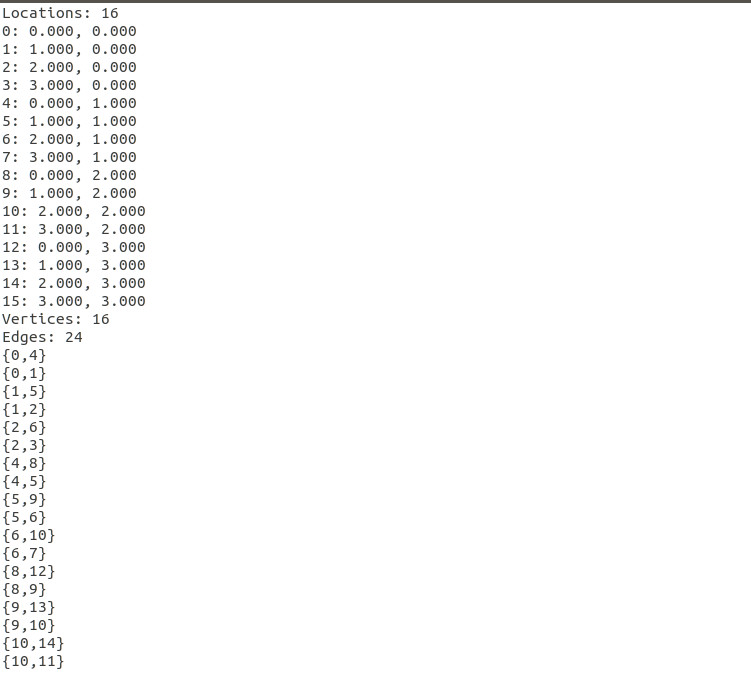
\includegraphics[scale=0.3]{Tests/testmap1.jpg}
	\caption[graph input data example]{graph input data example}\label{fig:float104}
\end{figure}

Agents parameters file incorporates such data as agent shape parameters, speed and acceleration. Additionally, it designates agent start location and agent target location.\ref{fig:float105}

\begin{figure}[H]
	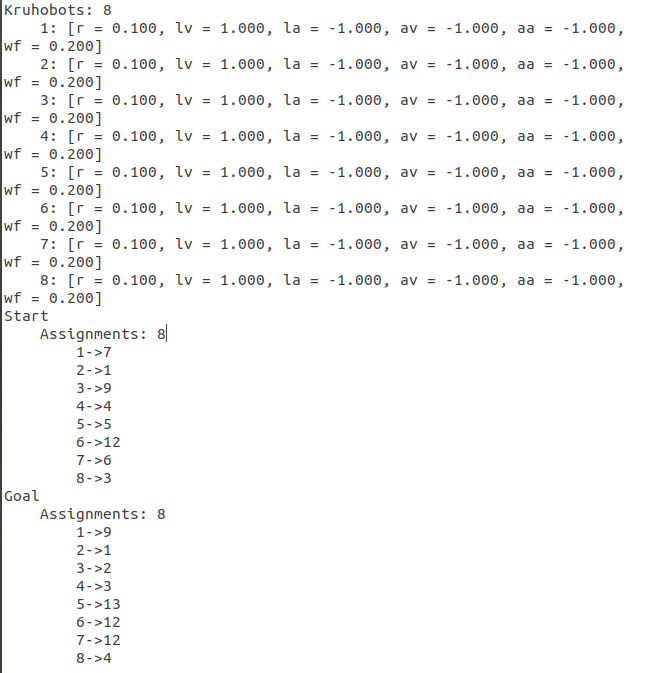
\includegraphics[scale=0.3]{Tests/testagent1.jpg}
	\caption[agents input data example]{agents input data example}\label{fig:float105}
\end{figure}


MAPF-R problem solution file gives data about agent schedule. For each agent it describes time intervals, starting location and finishing location. If starting and finishing location are the same vertex, it means that agent is waiting during that time interval.\ref{fig:float106}

\begin{figure}[H]
	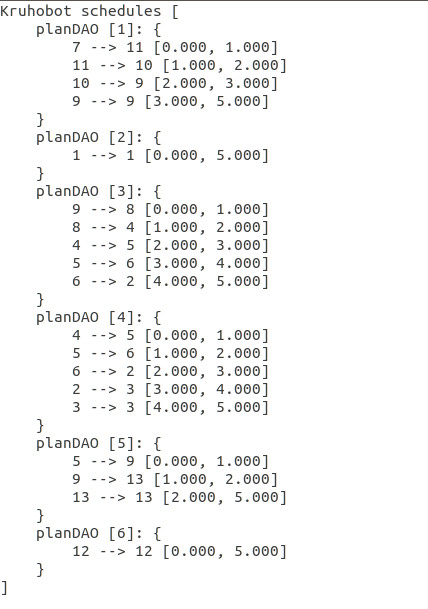
\includegraphics[scale=0.35]{Tests/testsolution1.jpg}
	\caption[solution input data example]{solution input data example}\label{fig:float106}
\end{figure}



\section{Technologies used}

The MAPF-R visualization tool ContinuousViz is designed as a client-based desktop PC application. It is an open-source application, meaning that other developers are approved to commit their changes to the project.

Since ContinuousViz was supposed to have real-time animations, we had to choose technology that enables programmer with high animation capabilities. We have chosen to use Java FX software platform, that function as GUI library for Java. It has support for web browsers and desktop PC on Linux, Microsoft Windows and MacOS.
GUI was created with Java FX Scene Builder, that enables dropping and dragging controls within application window frame. Afterwards that information is being converted into special XML file - FXML, that is code representation of GUI. 

Since Java FX is written in native Java, ContinuousViz code is likewise written in Java.

\section{Architectural design}

Since it was predetermined that ContinuousViz is going to be extended and updated, we have chosen modular architecture for the project. Modular architecture is an architectural design pattern, that is composed of distinct modules, which are connected with each other. Modules are defined as unique system units, that can be updated independently without affecting change in other modules. 

ContinuousViz has been devided into several modules, each responsible for a logically unified group of functions. User interaction with the system is conducted through graphic user interface, therefore it has been decided to place all elements of GUI into one module. This module is responsible for processing user's input and responding with an adequate output.

Next module stores business logic related functions. Overall logic manipulations, that involves changes in graph logic structure or agents logic structure, is placed into that module. 

Since it is presumed that visual representation of agent object and graph object could be potentially changed afterwards, all graphic objects will be placed into separate module as well as animation controllers. That separation allows alteration of objects visual forms without changing business logic or GUI manipulations. 

As far as statistical analysis is concerned, all functions that generate statistical data will be stored into separate module. This module will be coupled with business logic module, getting data about agent movements and generating statistical data out of it. 

Overall file input reading will be handled in separate module, so that it is possible to modify the way data is being read without changing how data is being processed afterwards. The next module will be managing video and photo processing, in case it will be needed to update video codecs or video/photo format\ref{fig:float4}. 

\begin{figure}
	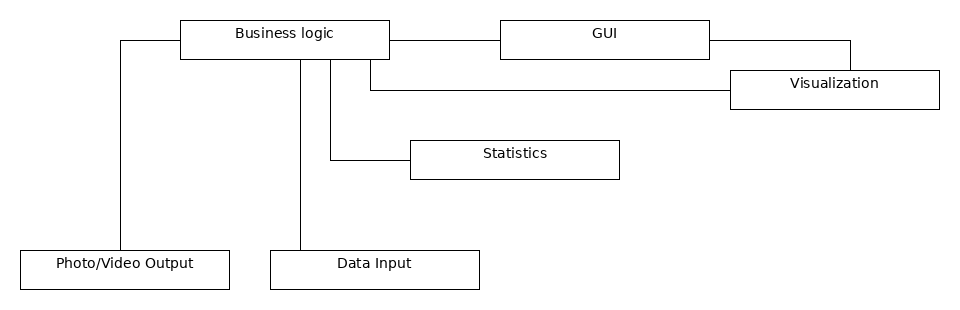
\includegraphics[scale=0.4]{Architecture.png}
	\caption[Architecture]{Architectural design}\label{fig:float4}
\end{figure}



\section{Component design}

Component design defines module components, logical or functional binary units that encapsulates behavior of a sowtware element. 

\subsection{Business logic module}

Business logic module contains components, that represents logical abstract entities  \ref{fig:float5}.Agent entity embodies parameters and behavior of Agent, such as identification, state, state change in timeline, starting location, target location. Agent entity is linked to Plan entity, which describes separate steps in timeline. Step entity has data about starting location, finishing location and time duration of the step. Alongside Agent entity, there is a Graph entity, which represents graph structure as well as incorporates vertex and edge entities. Both Agent and Graph entities are managed by special components, which are called AgentController and GraphController respectively. GraphController is linked to multiple AgentController components, since one Graph structure could possibly have multiple Agents moving on a Graph. On top of all that there is a MainController component that stores multiple GraphController components. It is responsible for manipulating overall business logic that is being executed within MAPF-R visualization tool.


\begin{figure}
	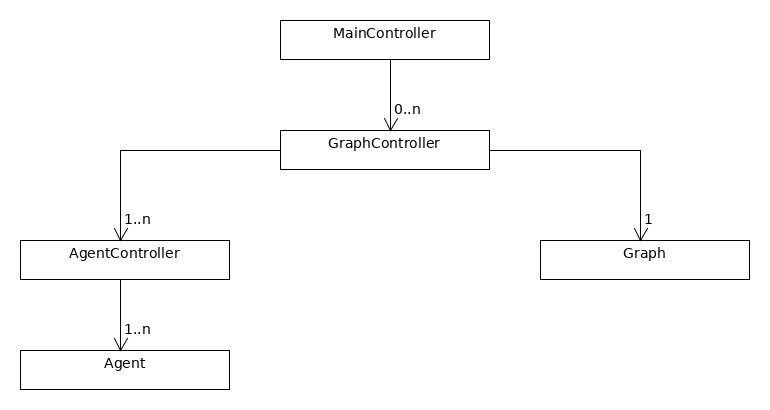
\includegraphics[scale=0.4]{BusinessLogic.png}
	\caption[Business logic]{Business logic module components}\label{fig:float5}
\end{figure}

\subsection{GUI module}

GUI module accumulates components, that controls defferent layouts of graphic user interfaces\ref{fig:float6}. MainGUI is the main component, which is responsible for main user activity, that involves uploading MAPF-R problem data, setting up and controlling visualization process. Besides that MainGUI component is responsible for activating other layouts, for instance, ColorChangerGUI component, which is aimed for setting up color parameters. In order to upload files LoadFileGUI component is being activated. LoadFileGUI component provides with file dialog so user could upload MAPF problem solution data. Aiming to visualize statistics data, it has been decided to design two separate layouts. SingleStatisticsGUI allows user to monitor statistical data for one single Agent, being speed change, location change, moving/waiting time ratio, etc.. Meanwhile DoubleStatisticsGUI showcases statistical data between two Agents, such as distance change, collision risk change, etc.. GroupStatisticsGUI enables to monitor statistical data of chosen group of Agents.     

\begin{figure}
	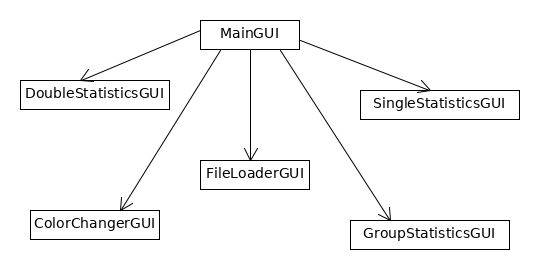
\includegraphics[scale=0.4]{GUIModuleComponents.png}
	\caption[GUI]{GUI module components}\label{fig:float6}
\end{figure}

\subsection{Statistics module}

Statistics module contains components, that generate statistical data\ref{fig:float7}. MovementAnalyzer component analyze agent changes in location during timeline for each millisecond of movement duration for each Agent. That data is stored in AgentMovement component, represented by array of SpaceTimeData entities. SpaceTimeData keeps data on location and time moment of Agent. After creating AgentMovement data set, MovementAnalyzer evaluates various statistical data out of AgentMovement and store it into StatisticsData component. Every type of statistical data is represented with its own component. CollisionData component keeps data about collisions between Agents, what time collision starts and what time collision ends between Agents. CollisionRiskData component keeps collision risk rate for every {Agent, Agent} pair for each millisecond of time duration, in the meantime DistanceData keeps distance data for every {pair, pair} for each millisecond of time duration. AgentTimeRatioData component indicates how much time Agent is in a certain state comparing to total time for all Agents in this certain state. ShortestDistanceData contains data about Agents, which move non-effectively on the graph. StatisticsData contains all those components and transport them into Business logic module. 

\begin{figure}
	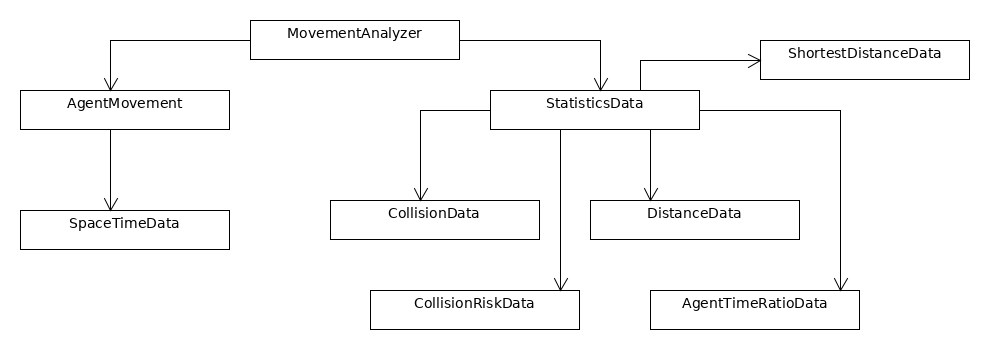
\includegraphics[scale=0.4]{StatisticsModuleComponent.png}
	\caption[Statistics]{Statistics module components}\label{fig:float7}
\end{figure}


\subsection{Visualization module component}

Visual elements module contains component, that is responsible for an animation - AnimationController. It creates an animation by generating \verb|key frames| for visual objects. Afterwards key frames are added to timeline. Timeline is controllable by GUI module components. In addition to that, visual elements module contains components, that represents Agent visual form and graph visual form - AgentVisual and GraphVisual respectively\ref{fig:float8}. Both those components are linked to Agent and Graph respectivly.

\begin{figure}
	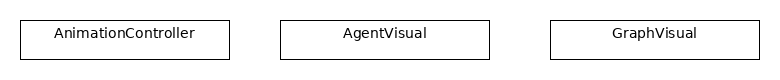
\includegraphics[scale=0.4]{Visualization.png}
	\caption[Visualization module components]{Visualization module components}\label{fig:float8}
\end{figure}


\subsection{DAO module}

DAO module contains components that are responsible for reading data and transform it into format, that could be used in other modules\ref{fig:float9}. DataRead component reads input files and add it to DataSet component. DataSet component contains data that is needed to create business logic entities.

\begin{figure}
	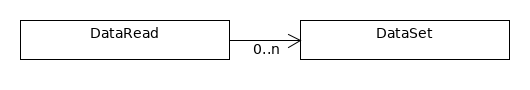
\includegraphics[scale=0.4]{DAO.png}
	\caption[DAO module components]{DAO module components}\label{fig:float9}
\end{figure}


\section{Test design}

\subsection{Incorrect input}

Incorrect input is designed to test if application is able to detect corrupt input data and react to it appropriately. Since there are three types of input files three respective types of test have been designed,
which are incorrect input of agents tests, incorrect graph input tests and incorrect input of agent plans. 

\subsubsection{Incorrect agents}

Incorrect agents test simulates various errors in agent description data. First type of error is wrong data format, for example, instead of numeric value data is presented as a string value.\ref{fig:float10} Second type is different file structure deviations: some obligatory parts are missing, there is no start or target destinations; incorrect order of data\ref{fig:float11}. Third type is logical error, for instance file header states a certain number of agents, however an actual number is less or more than has been stated.

\begin{figure}
	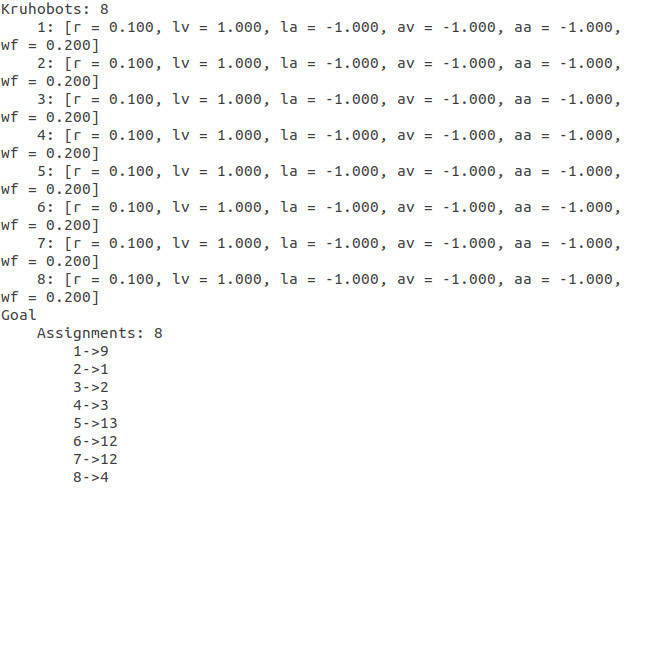
\includegraphics[scale=0.45]{Tests/testagent2.jpg}
	\caption[a.incorrect agents input example]{a.incorrect agents input example}\label{fig:float10}
\end{figure}

\begin{figure}
	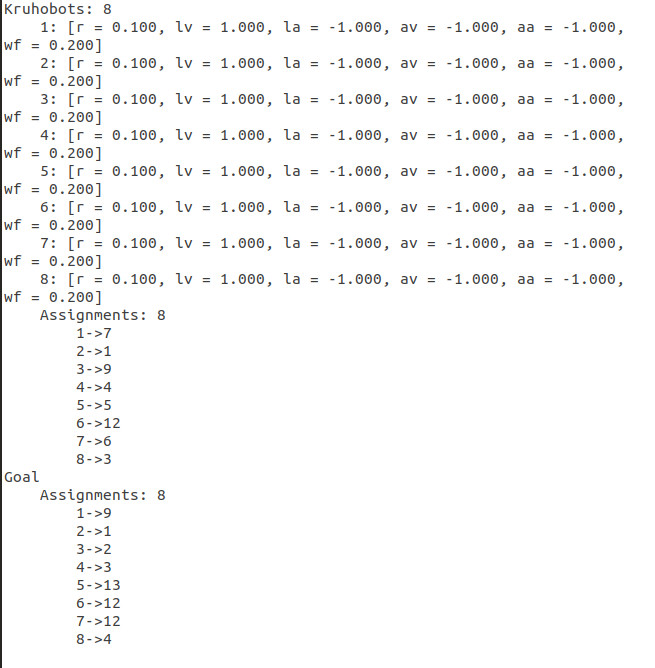
\includegraphics[scale=0.4]{Tests/testagent4.jpg}
	\caption[b.incorrect agents input example]{b.incorrect agents input example}\label{fig:float11}
\end{figure}


\subsubsection{Incorrect graph}

Incorrect graph tests represents test cases when graph data are corrupted in some way. Similar to incorrect agents input, errors could be divided into three subcategories: wrong data format, structural corruptions and logical errors\ref{fig:float12}. 

\begin{figure}
	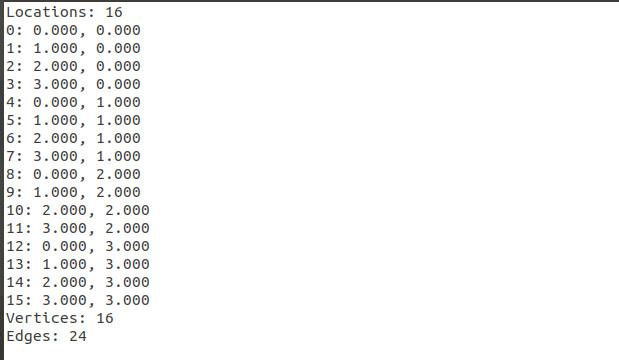
\includegraphics[scale=0.4]{Tests/testmap2.jpg}
	\caption[incorrect graph input example]{incorrect graph input example}\label{fig:float12}
\end{figure}


\subsubsection{Incorrect plans}

Incorrect plans tests simulate wrong data format and logical error, when there are more agents than plans. We assume, that every agent should be provided with a plan.

\subsection{Redundant solution}

Redundancy in solution can be divided into two main categories- occurence of collisions between agents and agent plan is ineffective.  

\subsubsection{Collision test}

Collision test is designed to check if application is able to detect collision events between agents. Plans input intentionally has collision situation implanted, which should be detected by application.

\subsubsection{Ineffective plans} 

Ineffective plan is a plan, which does not consist of the shortest paths possible(for example, result of BFS algorithm). Ineffective plans test is designed to check if application is able to assess the shortest distance possible by calculating path distance value(for example, using BFS algorithm). 

\chapter{MAPF-R visualization tool - ContinuousViz - developer manual}

In this chapter developer manual will be documented. More detailed documentation is presented on flash disk, attached to this thesis. It is intended to be read alongside source code, which makes it more comprehensible.

\section{Build}
 
General requirements for the MAPF-R visualization tool ContinuousViz project is JavaFX SDK at least version 11, therefore javafx-sdk-11.0.2 is included in distribution package. However, it is still needed to have JDK(Java Development Kit) installed. JavaFX 11 requires JDK 10, more recommended is JDK 11. JavaFX 11 builds on top of Java 11.

Additionaly FFmpeg library is needed for video capturing. FFmpeg is a free and open-source command-line tool for transcoding multimedia files, which has a set of shared audio and video libraries such as libavcodec, libavformat, and libavutil. With FFmpeg, it is possible to convert between various video and audio formats, set sample rates, and resize videos.

\subsection{Linux}

Usually, FFmpeg can be installed with the \verb|apt| package manager. First update packages list:
\begin{lstlisting}[language=bash]
sudo apt update
\end{lstlisting}
Then proceed with installing FFmpeg with following command:
\begin{lstlisting}[language=bash]
sudo apt install ffmpeg
\end{lstlisting}

To run \verb|jar| file type in command line:
\begin{lstlisting}[language=bash]
java --module-path javafx-sdk-11.0.2/lib/ --add-modules 
javafx.base, javafx.controls, javafx.fxml, javafx.graphics, 
javafx.media, javafx.swing, 
javafx.swt, javafx.web
-jar MAPF-R.visualization.tool.jar
\end{lstlisting}

, where javafx.* are modules that are used in this project. This command is written down in file \verb|run| file, therefore, you could just simply execute this file.

In case there is a freeze problem with GUI, type in command line:
\begin{lstlisting}[language=bash]
java -Dprism.order=sw -Dprism.verbose=true --module-path 
javafx-sdk-11.0.2/lib/ --add-modules  
javafx.base,javafx.controls,javafx.fxml,javafx.graphics,
javafx.media,javafx.swing,
javafx.swt,javafx.web 
-jar MAPF-R.visualization.tool.jar
\end{lstlisting}

, where -Dprism.order=sw and -Dprism.verbose=true are commands, which disable Hardware Graphics Acceleration(Prism) in JavaFX. 



\subsection{Windows}

To install FFmpeg on Windows, open the FFmpeg download site (for example,  https:\/\/ffmpeg.zeranoe.com\/builds\/ ) and download build. On your PC, open Advanced system settings and choose Environment Variables. Then choose Path variable and click New, there you should entry the path to FFmpeg library on your PC. At this point FFmpeg is activated in Command Promt.

To run \verb|jar| file on PC, open a \verb|notepad.exe|. Inside this file write down command line:
\begin{lstlisting}[language=bash]
java --module-path javafx-sdk-11.0.2/lib/ --add-modules 
javafx.base, javafx.controls, javafx.fxml, javafx.graphics, 
javafx.media, javafx.swing, 
javafx.swt, javafx.web
-jar MAPF-R.visualization.tool.jar
\end{lstlisting}   

Afterwards save this file with extension \verb|.bat| and copy it to the directory with \verb|jar| file. Double click it to run application. 

\section{Business logic}

\begin{figure}
	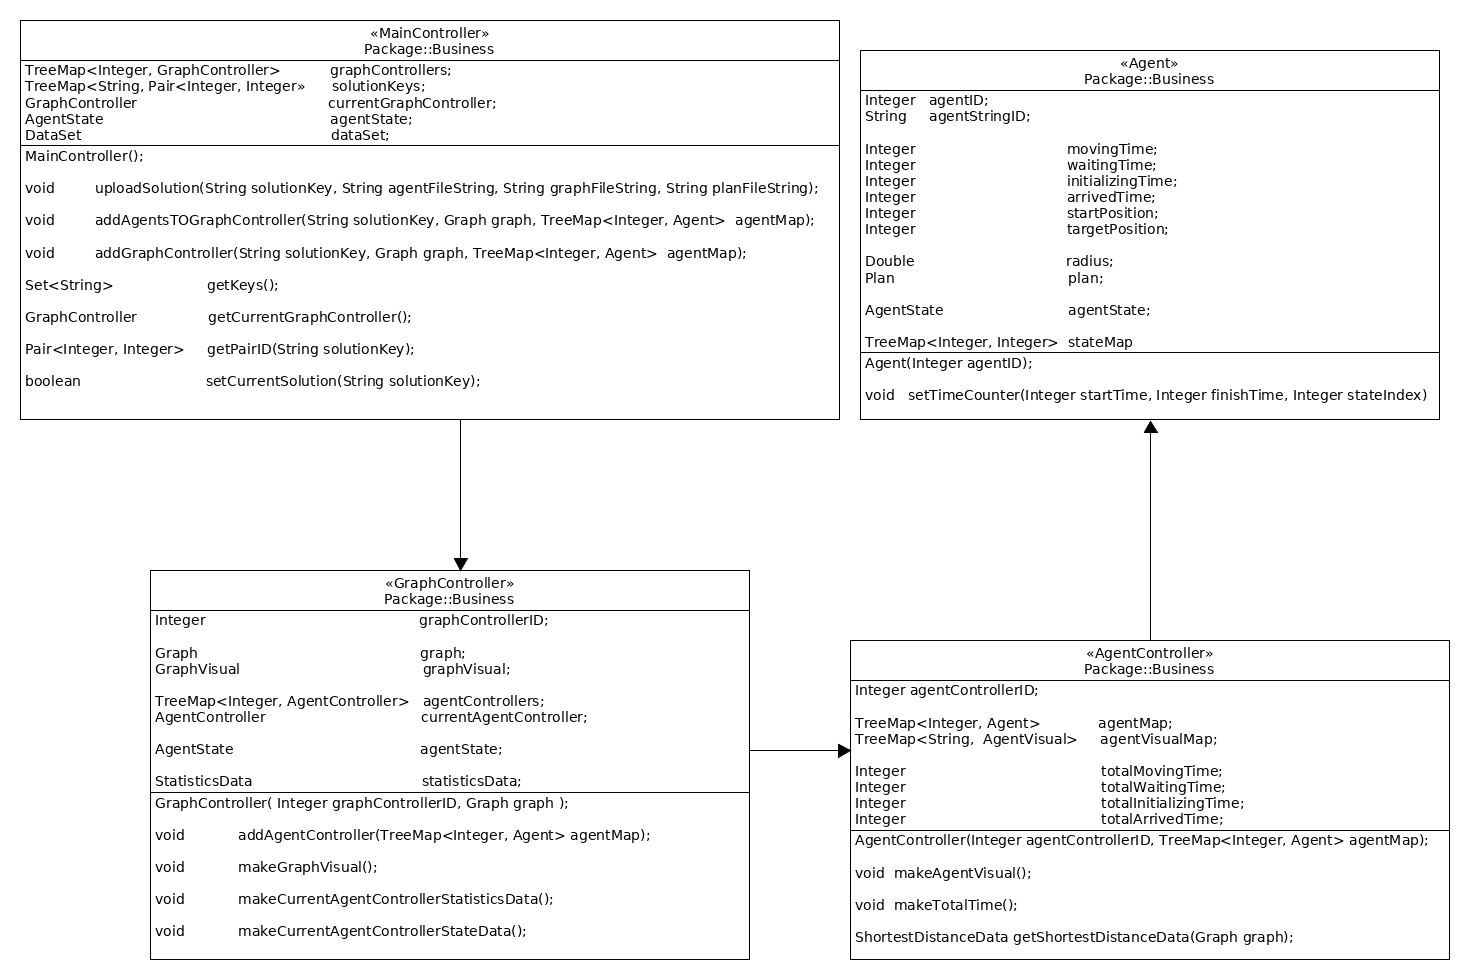
\includegraphics[scale=0.29, center]{diagrams/Business.png}
	\caption[Business logic module class diagram]{Business logic module class diagram}\label{fig:float13}
\end{figure}

\subsection{Agent}
Agent class represents a single Agent object that is moving on the Graph. Agent class has following parameters Integers agentID, which is unique Agent identifier, startPosition, targetPosition - indexes of start location and target location. Schedule of Agent movement is prescribed in Plan plan variable.

Integer values \verb|movingTime|, \verb|waitingTime|, \verb|initializingTime|, \verb|arrivedTime| are displaying how much summarized time Agent spends in AgentState MOVING, WAITING, INITIALIZING, ARRIVED. 

Agent class has variable
\begin{description}
\item[TreeMap\textless Integer, Integer\textgreater stateMap] where key is  a time moment of movement and a value is AgentState identification index, suggesting in which state Agent is in at that particular moment of time
\end{description}

Public method setState(Double startTime, Double finishTime, Integer stateIndex) puts values into stateMap for each millisecond between finishTime and startTime. It also calls private method setTimeCounter(Integer startTime, Integer finishTime, Integer stateIndex), that adds delta between  \verb|finishTime| and \verb|startTime| to corresponding variables: movingTime, waitingTime, initializingTime or arrivedTime.

\subsection{AgentState}

AgentState class is responsible for establishing a correlation between String and Integer values of state. For instance, value 0 indicates that Agent is in state \verb|Initializing|, etc.

\subsection{Plan}
Plan class represents a schedule of Agent movements on a Graph. Plan class has a private variable:
\begin{description}
\item[List\textless Step \textgreater stepList] which stores Steps taken by Agent
\end{description}

Public method addStep(TimeInterval timeInterval, int from, int to) create an instance of Step and add it to stepList. Public method getStepList() returns stepList. 

\subsection{Step}
Step class represents a structural unit of an Agent movements on a Graph. Step class has following private variables: 
\begin{description}
\item[TimeInterval timeInterval] which is a time duration of Step
\item[Integer from] index of start Vertex that is involved in Step
\item[Integer to] index of finish Vertex that is involved in Step
\end{description}

\subsection{TimeInterval}
TimeInterval class represents delta between start time moment of movement and finish time moment of movement. TimeInterval class has two private variables: Double startTime and Double finishTime.
Public method getValue() returns delta value between \verb|startTime| and \verb|finishTime|. 

\subsection{Vertex}
Vertex class represents a vertex on a Graph. Vertex class has following parameters Integer vertexIndex( unique Vertex identifier), Double xCoordinate and Double yCoordinate, that represents Vertex location on Cartesian coordinates system.

\subsection{Edge}
Edge class represents an edge on the Graph. Edge class has two private Integer variables fromIndex, toIndex, which are indexes of Vertices, connected by Edge.

\subsection{Graph}
Graph class represents a graph on which Agents are moving. Graph class has two private variables:
\begin{description}
\item[List\textless Edge\textgreater edges] which is the List of Edges
\item[TreeMap\textless Integer, Vertex\textgreater verticesMap] where a key is a Vertex index and a value is a Vertex object with this index 
\end{description}


Public method addEdge(int fromIndex, int toIndex) adds new instance of Edge to edges.
Public method addVertex(int index, double xCoordinate, double yCoordinate) creates a new Vertex instance and add it to verticesMap, where Vertex identifier is a key and Vertex is a value.

Public method getEdges() returns edges. Public method getVerticesMap()
returns verticesMap. Public method getVertices() creates and returns List \textless Vertex\textgreater vertices. Method getVertices() is called when time complexity O(n) is acceptable, method getVerticesMap() is called when time complexity O(log n) is acceptable. 

Public method equals(Graph anotherGraph) returns boolean value and checks if two graph are identical, i.e. has same Vertex and Edge structure.

\subsection{AgentController}

AgentController class represents a group of Agents, that are corresponding to a current solution. AgentController class main objectives are to store Agents, to convey operations with Agents and to modificate parameters of Agents.

AgentController class has following private variables:
\begin{description}
\item[TreeMap \textless Integer, Agent \textgreater agentMap] where a key is Agent identification and value is Agent.
\item[TreeMap\textless String,  AgentVisual\textgreater  agentVisualMap] where key is Agent identification as String value, and value of the map is AgentVisual.
\end{description}


Private method makeAgentVisual() iterates through agentMap, generates AgentVisual for each Agent and puts it into agentVisualMap. Public method getAgentVisual(Integer agentID) returns AgentVisual that corresponds to Agent with given agentID.

Public method setAgentState(...) invokes public method Agent.setState(Double startTime, Double finishTime, Integer stateIndex) for Agent that corresponds to agentIndex. Public method getAgentState(Integer agentIndex, Integer time) returns Integer AgentState index, which coresponds state of Agent with agentIndex in time moment.

\subsection{GraphController}

GraphController class represents a structure of Graph and its group of Agents. GraphController has private variables Graph graph and GraphVisual graphVisual. Private method makeGraphVisual iterates through Edges and Vertices of Graph and generates GraphVisual value.  

GraphController class has private variable TreeMap \textless Integer, AgentController \textgreater AgentContollers, that represents groups of Agents that correspond to that solution. Private variable AgentController currentAgentController corresponds to current solution, that has been uploaded. Public method setCurrentAgentController(Integer agentControllerID) sets an AgentController that has identifier agentControllerID as currentAgentController. Public method addAgentController(TreeMap agentMap) creates a new instance of AgentController with agentMap, sets it as a default currentAgentController and calls private method makeCurrentAgentControllerStateData().

Private method makeCurrentAgentControllerStateData() iterates through each Agent from currentAgentController. For each agent it gets Plan and iterates through each Step of Plan and identifies AgentState for given Step. When AgentState is identified method calls AgentController.setAgentState(...) method to set AgentState. Public method getAgentState(...) returns AgentState index from currentAgentController. 

Public method getGraphStatisticsData()  returns StatisticsData object. getGraphStatisticsData() invokes private method makeCurrentAgentControllerStatisticsData(), which generates StatisticsData relevant for graph and currentAgentController.

\subsection{MainController}

MainController class controls operations with GraphControllers as well as other business logic operations. It has following private variables: TreeMap \textless Integer, GraphController\textgreater graphControllers, where key is GraphController identifier and value is GraphController,  GraphController currentGraphController, that corresponds to current uploaded solution.

MainController class has private variable TreeMap \textless String, Pair \textless Integer, Integer\textgreater\textgreater   solutionKeys, where key String is a unique identifier of uploaded solution and Pair \textless Integer, Integer\textgreater is a pair of GraphController and AgentController identifiers.

Public method setCurrentSolution(...) gets pair of GraphController and AgentContoller idenifiers - Pair \textless Integer, Integer\textgreater pairID, using private method getPairID(...). Afterwards, it sets currentGraphController, that has identifier pairID.getKey(), and currentAgentController, that has identifier pairID.getValue(). Public method getCurrentGraphController() returns currentGraphController, which corresponds to current uploaded solution.

MainController class has private variable DataSet dataSet, that contains data from input files. Public method uploadSolution(...) calls public method DataSet.makeDataSet(...) to read relevant data from given files. Finally, it invokes private method addGraphController(...).

Private method addGraphController(...) creates a new instance of GraphController and AgentController. New instance of GraphController is added to graphControllers. Additionaly, solutionKey and graphController, agentContoller identifiers are added to solutionKeys.

\section{Statistics}

\begin{figure}
	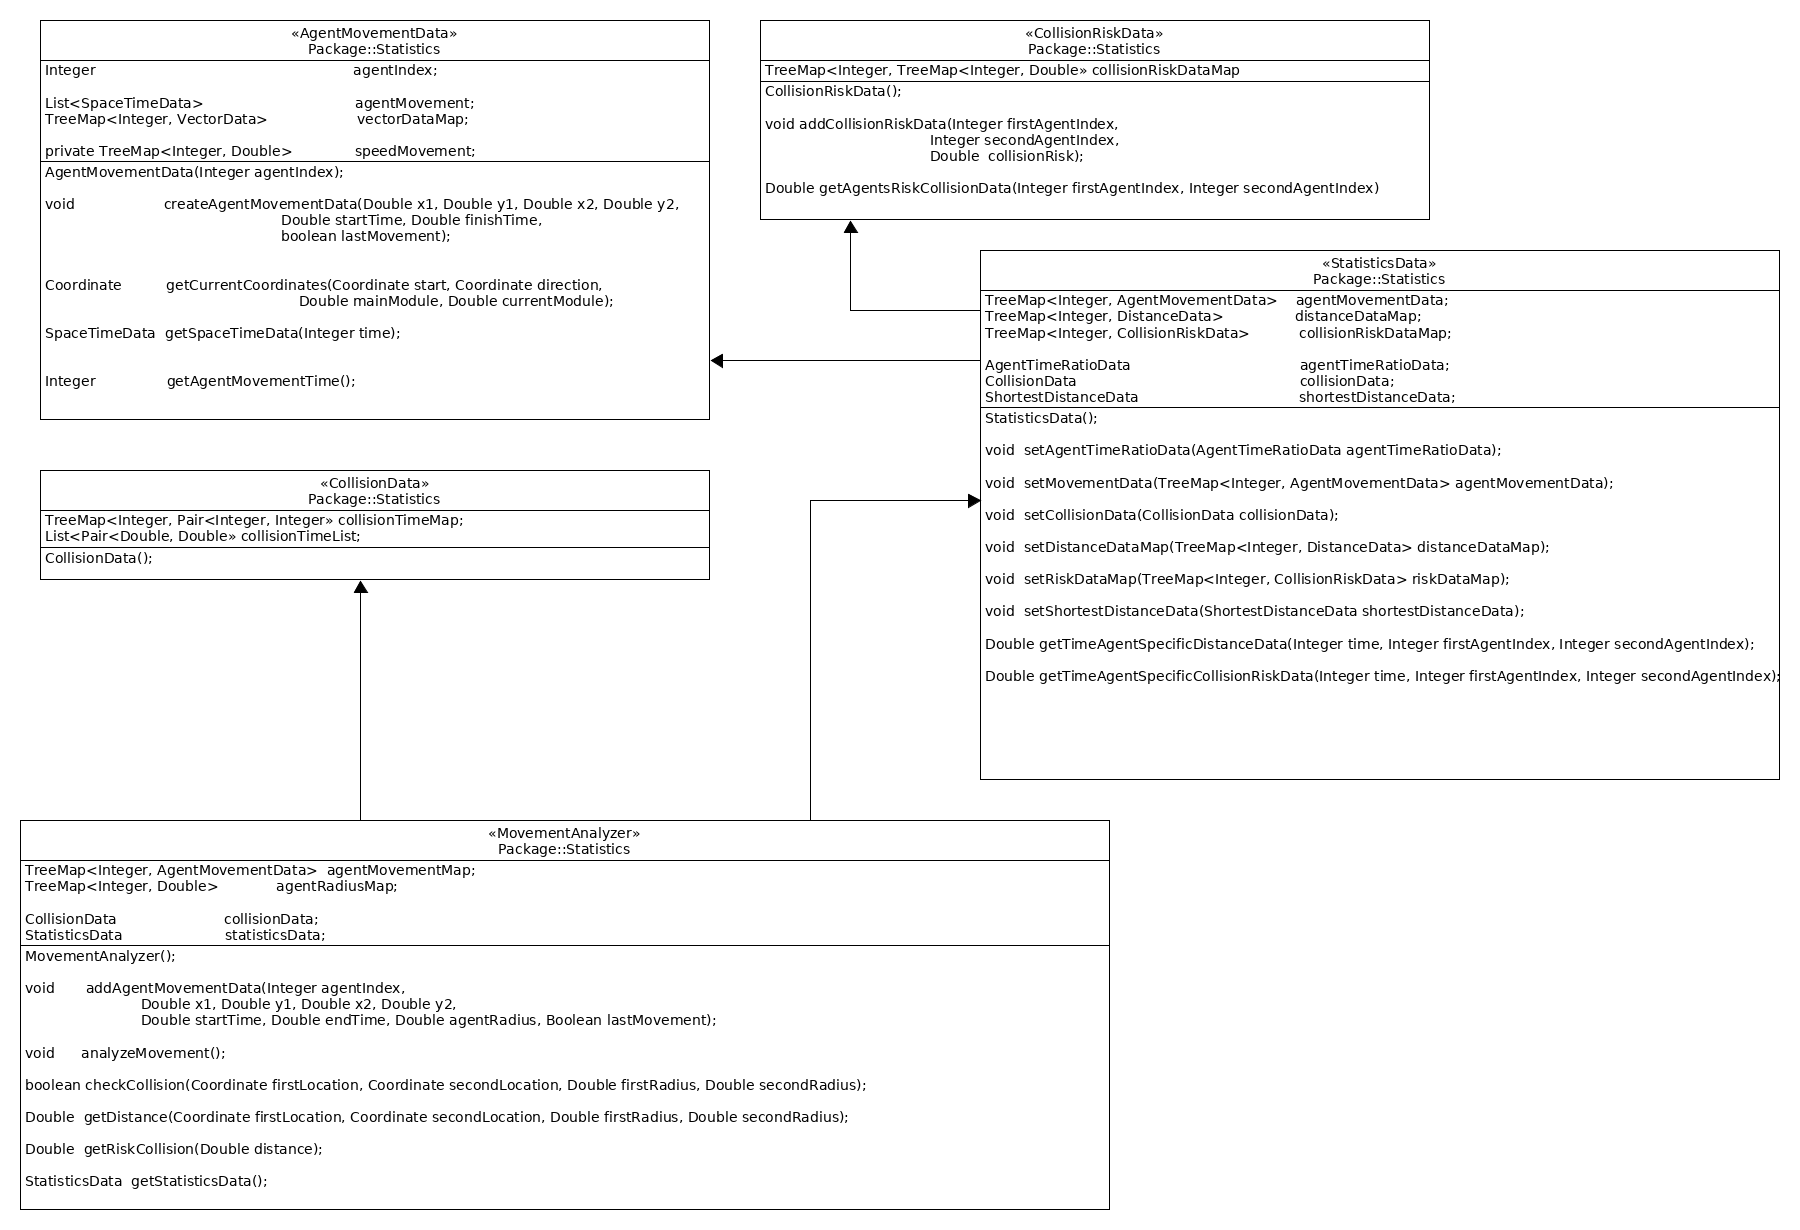
\includegraphics[scale=0.25]{diagrams/Statistics.png}
	\caption[Statistics module class diagams]{Statistics module class diagram}\label{fig:float14}
\end{figure}


\subsection{SpaceTimeData}

SpaceTimeData class keeps data about Agent position in time and space. It has private variable Coordinate space, that contains Agent coordinates, and private variable Double time.

\subsection{Coordinate, VectorData}

Coordinate class represents coordinate value within cartesian coordinate system. It has two private variables:
Double xCoordinate, Double  yCoordinate. 

VectorData class keeps data of movement vector. It has three private variables Coordinate vectorStart, vector starting point, vectorFinish, vector finishing point, and vectorDirection, which is coordinates representation of vector direction.

\subsection{AgentMovement}

AgentMovementData class has private variable:
\begin{description}
\item[List \textless SpaceTimeData\textgreater agentMovement] which stores data for an Agent about its movement for each millisecond of movement duration
\end{description}

Public metod createAgentMovementData(...) generates movement data for an Agent. It creates an instance of VectorData class using coordinates x1, y1, x2, y2. Based on vector lenght and duration of movement, which is delta between finishTime and startTime, it evaluates Agent speed. Then it iterates through each millisecond of movement duration and defines length, that Agent has accomplished by this particular moment. Using this length value, method defines current coordinates of Agent. Based on that data a new instance of SpaceTimeData is created and added to AgentMovement.

\subsection{DistanceData}

DistanceData class keeps data about distance between all possible pair combinations of Agents. It has private variable:
\begin{description}
\item[TreeMap\textless Integer, TreeMap\textless Integer, Double\textgreater\textgreater distanceDataMap] where key is an index of Agent, and value is a map with the key index of a second Agent and  with a value of a distance between them
\end{description}


\subsection{CollisionData}

CollisionData class keeps data about collision events that happened between Agents.
It has private varibles:  
\begin{description}
\item[List \textless Pair\textless Double, Double\textgreater\textgreater collisionTimeList] stores data about starting time moment and ending time moment of the collision event
\item[TreeMap \textless Integer, Pair\textless Integer, Integer\textgreater\textgreater collisionMap] stores data about the collision event. A Key is an index of Pair\textless Double, Double\textgreater in collisionTimeList, value is a pair of Agents, that are involved in the collision event
\end{description}

\subsection{CollisionRiskData}

CollisionRiskData class keeps data about risk rate of potential collision between all possible pair combinations of Agents. It has private variable:
\begin{description}
\item[TreeMap\textless Integer, TreeMap\textless Integer, Double\textgreater\textgreater collisionRiskDataMap] where key is an identification of Agent and value is a map, with a key index of another Agent and with a value of a collision risk rate
\end{description}

\subsection{AgentTimeRatio}

AgentTimeRatio class keeps data about how much time Agent spends in particular AgentState. It has private variables:
\begin{description}
\item[Integer movingTime] time spent in the state Moving (moving between vertices)
\item[Integer waitingTime] time spent in the state Waiting (waiting on a vertex)
\item[Integer initializingTime] time spent in the state Initializing (standing on the start vertex, movement has not been started yet)
\item[Integer arrivedTime] time spent in the state Arrived (standing on the target vertex, movement has been finished already)
\end{description}


\subsection{AgentTimeRatioData}

AgentTimeRatioData class keeps AgentTimeRatio objects for each Agent in the private variable:
\begin{description}
\item[TreeMap\textless Integer, AgentTimeRatio\textgreater agentTimeRatioTreeMap]  where key is an identification of Agent and value is an instance of AgentTimeRatio class
\end{description}


\subsection{ShortestDistanceData}

ShortestDistanceData class keeps data about Agents, which has non-optimal path distances. It has method getBFSDistance(...) that calculates shortest distances between all possible pairs of vertices on the graph using BFS algorithm. In addition, it has method getActualDistance(...), that calculates actual distance that Agent traverses from a start position to its target position. Method runDistanceTest() invokes compares the shortest distance with an actual distance, in case those distances are not equal the actual distance is not optimal. ShortestDistanceData keeps data in private variable:
\begin{description}
\item[List\textless Integer \textgreater notShortestDistanceList] which is a list of Agent indexes that have non-optimal distance values.
\end{description}



\subsection{StatisticsData}

StatisticsData class transports instances of AgentTimeRatioData, DistanceData, CollisionData, CollisionRiskData and ShortestDistanceData from statistics module to business logic module.  

\subsection{MovementAnalyzer}

AgentAnalyzer class has following private variables:
\begin{description}
\item[TreeMap \textless Integer,  AgentMovementData\textgreater agentMovementMap] key is Agent index and value is an instance of AgentMovementData
\item[TreeMap \textless Integer, Double\textgreater agentRadiusMap] keeps data about Agent radius, this data is used in order to assess distance between Agents
\item[CollisionData collisionData] stores all data concerning collisions between Agents. Private method getRiskCollision(Double distance) returns Double value, which is a rate of collision risk between two Agents
\item[StatisticsData statisticsData] stores all statitical data generated in method analyzeMovement()
\end{description}

Private method analyzeMovement() convey analysis of Agents movement. In order to store all generated data following variables are implemented:
\begin{description}
\item[TreeMap \textless Integer, DistanceData\textgreater distanceDataMap] stores all distance related data for each millisecond of movement duration. Key is millisecond index, value is an instance of DistanceData  
\item[TreeMap \textless Integer, CollisionRiskData\textgreater collisionRiskDataMap] stores all collision risk related data for each millisecond of movement. Key is millisecond index, value is an instance of CollisionRiskData
\end{description}	

Side-note: Milliseconds are converted into Integer variables in order to avoid precision-based errors assosiated with Double values.

In order to generate combination type 'all Agents with all Agents' method implicates Agent itaration inside Agent iteration. With given pair of Agents method iterates through each millisecond of the movement. For each millisecond method evaluates current distance in Agents pair - Double currentDistance, current rate of collision risk in Agents pair - Double currentRiskCollision. Using currentDistance value a new instance of DistanceData is created and added to distanceDataMap. Using currentRiskCollision value a new instance of CollisionRiskData is created and added to collisionRiskData. 

Inside milliseconds iteration private method checkCollision() is called to verify if collision event has happened. If it has, boolean variable collisionActive is set to be true, current millisecond is written into Double startTime. When method checkCollision() returns false value and collisionActive is true, it means that collision event has finished. Value collisionActive is set to be false, current millisecond is written into Double finishTime. Values startTime and finishTime are added to collisionTimeList as Pair of Doubles. After that, new entry is added to collisionMap. 

When all milliseconds are iterated for all possible pair combinations of Agents, 
collisionTimeList and collisionMap are added to collisionData. Finally,
collisionData, agentMovementMap, distanceDataMap, collisionRiskDataMap are added to statisticsData.

\section{Visualization}

\begin{figure}
	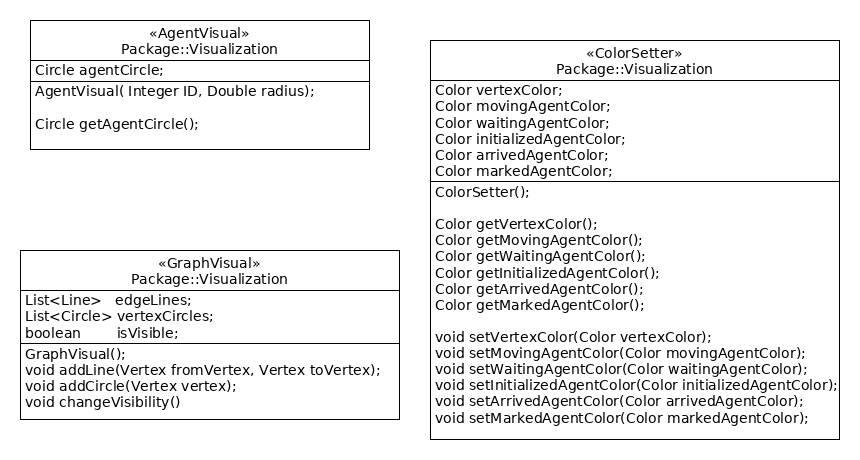
\includegraphics[scale=0.3, left]{diagrams/Visualization2.png}
	\caption[a. Visualization module class diagram]{a. Visualization module class diagram}\label{fig:float15}
\end{figure}


\subsection{AgentVisual}

In this implementation of MAPF-R visualization tool, it is considered that Agent has a shape of a circle, therefore AgentVisual class has visual object Circle agentCircle, that represents Agent in visualization. In constructor method AgentVisual() Agent identifier is set to Circle object - agentCircle.setId(ID.toString()), which allows to get right Circle object for Agent. Such parameters as radius and visibility are also set in costructor method AgentVisual().

\subsection{GraphVisual}
GraphVisual class contains List of Lines and List of Circles, that represents Edges and Vertices in visualization. Line is created in public method addLine(Vertex fromVertex, Vertex toVertex), where Vertices fromVertex and toVertex define coordinates of Line points. Circle, that represents Vertex, is created in method addCircle(Vertex vertex), where vertex defines coordinates of Circle center point. Public method changeVisibility() iterates through all Lines and Circle and switch their visibility status.           

\subsection{ColorSetter}

CollorSetter class transports color values stored in Colors variables: movingAgentColor, waitingAgentColor, initializedAgentColor, arrivedAgentColor, markedAgentColor, vertexColor. 

\subsection{AnimationController}

AnimationController class is responsible for animating visualized solution. It has Timeline variable - timeline. Timeline is defined by one or more KeyFrames object, which are being sequentially processed in time. Public method initializeTimeline(GraphController graphController, AgentController currentAgents) calls internal private method getKeyFrames(GraphController graphController, AgentController currentAgents), that iterates through Agents getting for each Agent its plan of movement and visual representation and send them to internal private method moveTimeline(Circle agentCircle, Plan plan, TreeMap \textless Integer, Vertex\textgreater verticesMap). In moveTimeline() method KeyFrames for Circle agentCircle according to Plan plan are being generated.

Public method playAnimation() plays animation at a current time position.
Public method playAnimationFrom(Number timePosition) plays animation from timePosition value. Public method pauseAnimation() pauses animation, meanwhile public method stopAnimation() stops it and resets animation speed back to normal in case it has been changed. Public methods speedUpAnimation(), slowDownAnimation() alter animation speed. Public methods forwardDirectionAnimation(), backwardDirectionAnimation() alter direction of movement - forwards or backwards respectively.


\begin{figure}
	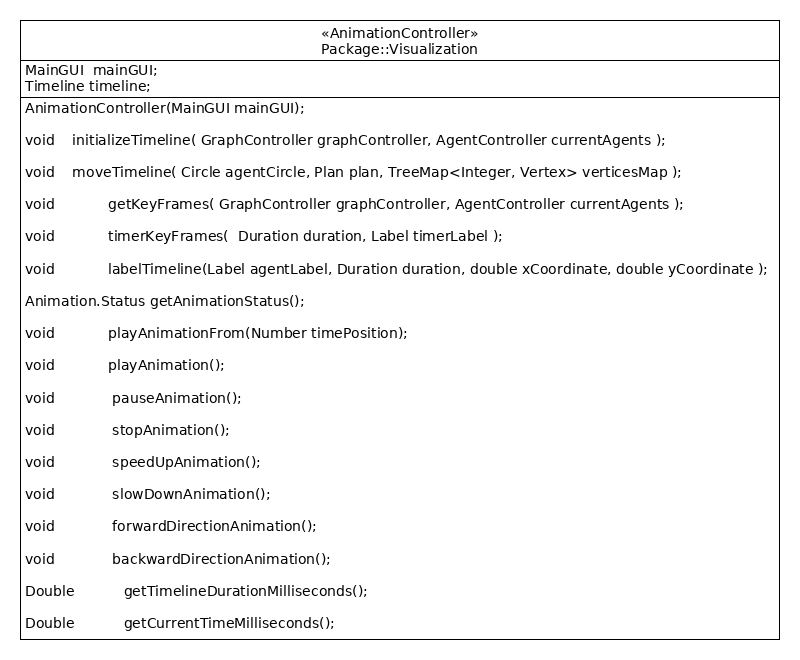
\includegraphics[scale=0.3, left]{diagrams/Visualization1.png}
	\caption[b. Visualization module class diagram]{b. Visualization module class diagram}\label{fig:float16}
\end{figure}


\section{GUI}

StartGUI class extends Application class, which starts overall application by invoking start() method. In this method stage for Main.fxml is created. Main.fxml is controlled by MainGUI class, inside which majority of graphic user interface is managed. MainGUI class has singleton MainController variable - mainController, that controlls all business processes. GUI accepts user signals and addresses them to mainController. GUI functionality can be divided into several subsections:

\subsection{Uploading solution}

GUI nodes that are responsible for uploading solution are button setSolutionButton and TreeView solutionTree, where all uploaded solutions are displayed.

By clicking setSolutionButton class MainGUI method setFileLoader() is called, which activates LoadFile.fxml, controlled by LoadFileGUI class. In LoadFileGUI class there are three FileChooser variables: agentFileChooser, graphFileChooser, planFileChooser. Those variables are respobsible for file dialogue for each respective type of file. In file dialogue user inputs paths to files, which are written down into string variables agentFileString, graphFileString, planFileString. In addition to that user inputs solution name, that is stored into string variable SolutionKey, which serves as a solution unique identifier. Those string variables are parameters for method setSolution() in MainGUI class, that uploads solution. Meanwhile solutionTree node is updated by calling method setSolutionList() in MainGUI class, which adds newly uploaded solution to TreeView.

\subsection{Starting and controlling solution visualization}

StartVisualizationButton node is responsible for starting solution visualization. It invokes method startVisualization() in MainGUI class, which gets unique identifier - solutionKey from chosen solution in TreeView node. In startVisualization() private method uploadChosenSolution() is called, which asks mainController to set solution that has unique identifier - solutionKey.

After solution has been set, inside startVisualization() method private method visualizeSolution() is called, which gets visual elements of agents(circle for example) and graph(lines and circles) from mainController and puts it on \verb|mainVisualPane| node. Additionally, in startVisualization() method a new instance of AnimationController class, that is responsible for animating visual elements, is created. 

In startVisualization() private method startStatistics() is invoked in order to set up and update visual representation of statistical data.

Finally, in startVisualization() method private method initializeConotrols() method is called, that prescribes actions to nodes playButton, stopButton, forwardButton, backwardButton, slowDownButton, speedUpButton, it also initializes Slider nodes - timelineSlider and rotationSlider. 

\subsection{Setting up color palettes interface}

Node changeColorButton call setColorChanger() method in MainGUI class, that activates layout ColorChanger.fxml, that is controlled by ColorChangerGUI class. ColorChangerGUI has several ColorPicker variables: vertexColor, arrivedAgentColor, initializedAgentColor, waitingAgentColor, movingAgentColor, markedAgentColor. After values of ColorPicker variables have been set, they are set in ColorSetter class.  


\subsection{Setting up statistics interfaces}

Node singleAgentStatisticsButton calls setSingleAgentStatistics() method in MainGUI class, that activates layout SingleAgentStatistics.fxml, controlled by SingleAgentStatisticsGUI class. In method setSingleAgentStatistics() public method SingleAgentStatisticsGUI.setStatisticsData() is called -  it sets up StatisticsData variable - statisticsData, which is get from mainController varibale in MainGUI. 

Node doubleAgentStatisticsButton calls setDoubleAgentStatisitcs() method in MainGUI class, that activates layout DoubleAgentStatistics.fxml, controlled by DoubleAgentStatisticsGUI class. In method setDoubleAgentStatistics() public method DoubleAgentStatisticsGUI.setStatisticsData() is called -  it sets up StatisticsData variable - statisticsData, which is get from mainController varibale in MainGUI.

Method startStatistics() is called inside startVisualization() method. Inside this method ScheduledExecutorService is set. SceduledExecutorService extends ScheduledService, that is able to schedule commands to run after a given delay, i.e. execute periodically. In startStatistics() method scheduled service updates visual representation of statistical data every second of animation. Depends on what layout is activated, service sends current time of animation by calling public method SingleAgentStatisticsGUI.updateCurrentTime(Integer time) or DoubleAgentStatisticsGUI.updateCurrentTime(Integer time). Variable \verb|time| is a key, with which statistical data is get from statisticsData variable and visualized on layouts.

\subsection{Converting visualization into photo/video format}

Private method takeSnapshot() invokes an instance of PhotoOuputController class, that
creates a photo image. Mathod takeSnapshot() sends \verb|mainVisualPane| node, which contains graph and agents visualization, as an argument of  PhotoOutputController.takeSnapshot(String snapName, Node node) method. In case SingleAgentStatistics.fxml layout or DoubleAgentStatistics.fxml layout are activated, method sends those nodes as an arguments as well.

Private method takeVideo() invokes an instance of VideoOutputController class, which starts video capturing process. If video capturing process has already been activated, method stops video capture process. 

\begin{figure}
	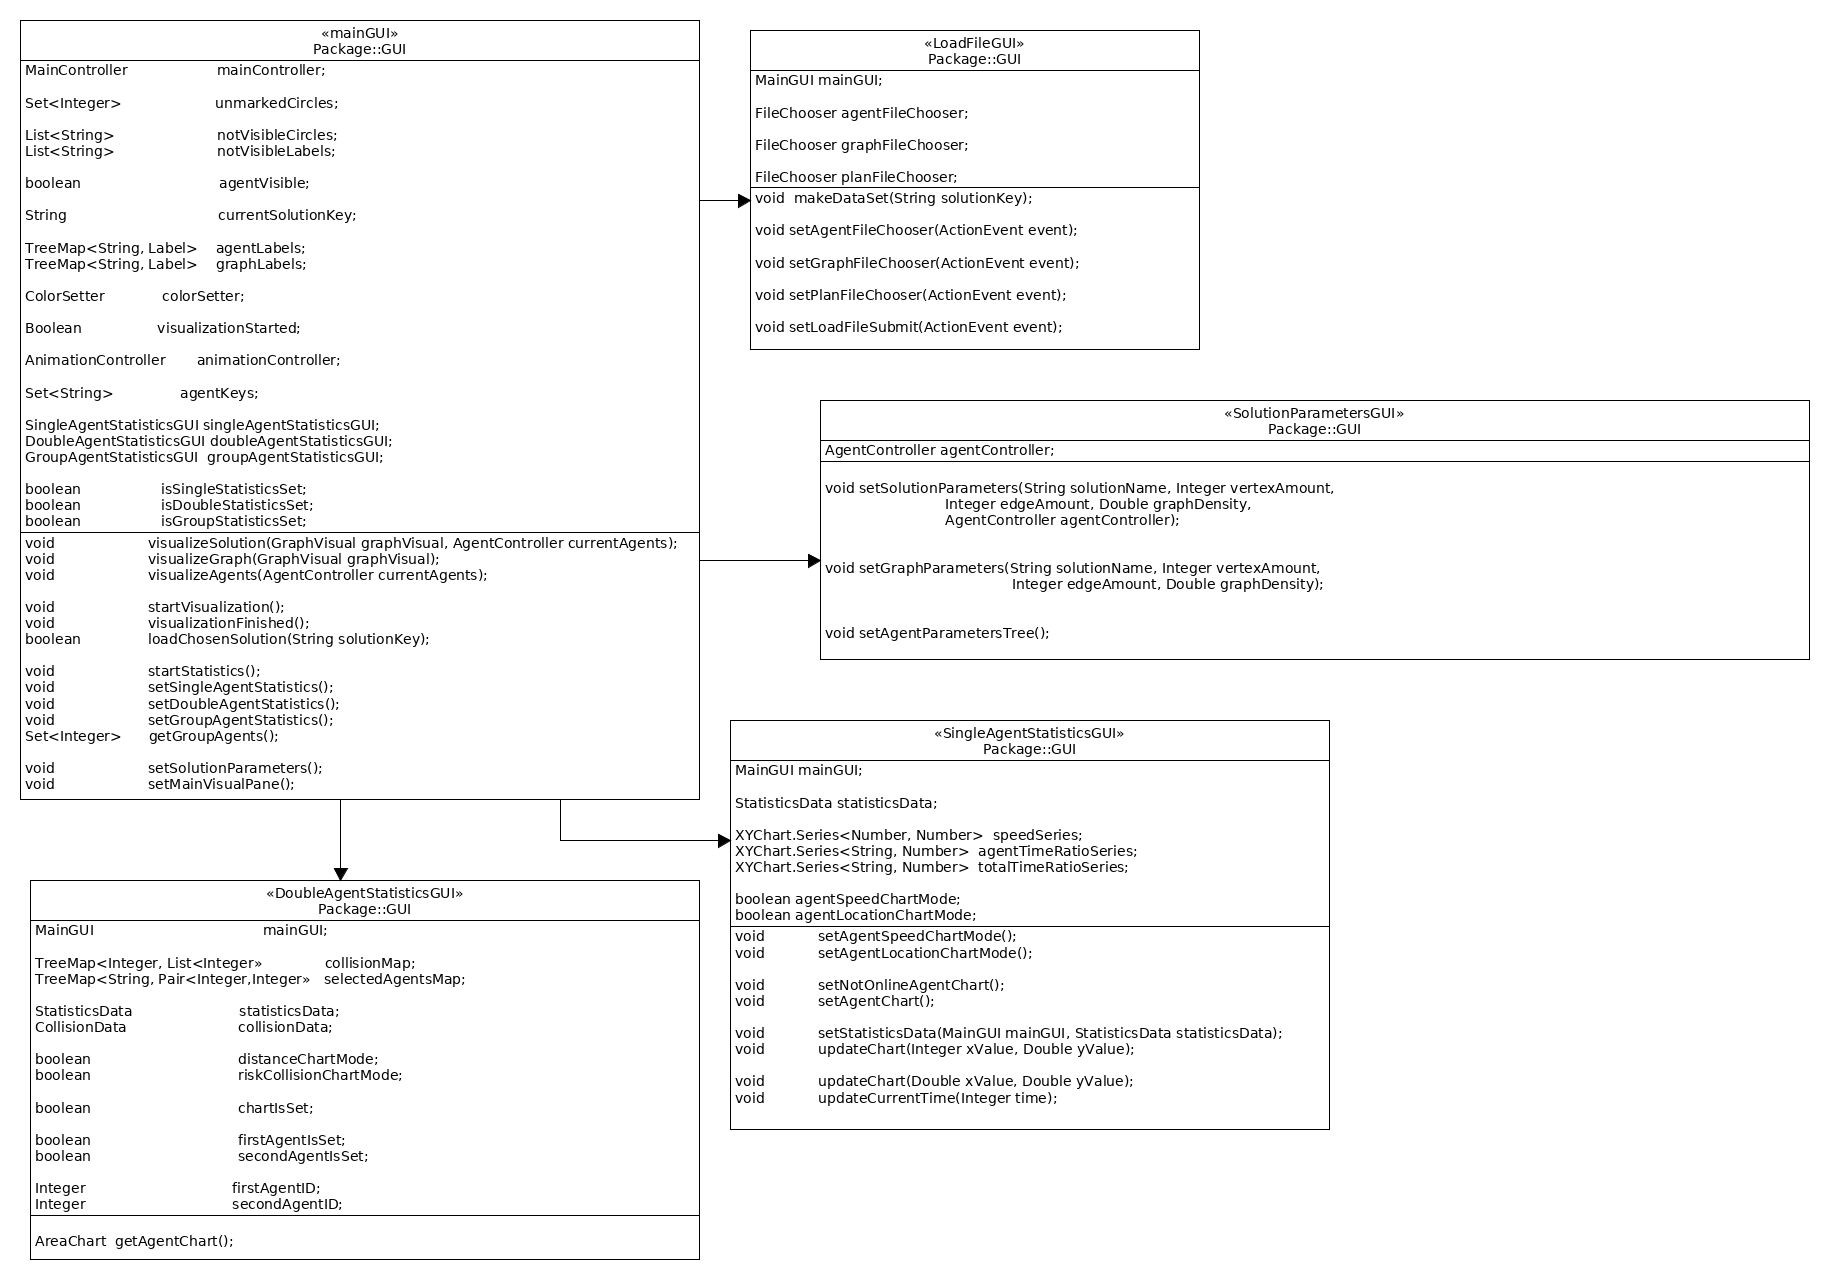
\includegraphics[scale=0.26, left]{diagrams/GUI.png}
	\caption[GUI module class diagram]{GUI module class diagram}\label{fig:float17}
\end{figure}

\section{DAO}

\begin{figure}
	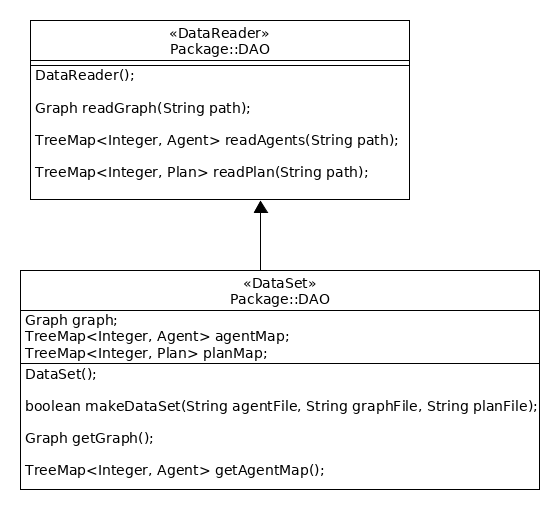
\includegraphics[scale=0.26, center]{diagrams/DAO.png}
	\caption[DAO module class diagram]{DAO module class diagram}\label{fig:float18}
\end{figure}

\subsection{DataReader}

DataReader class reads data from input files. It has following public methods:
\begin{description}
\item[Graph readGraph(String path)] reads file, that describes graph structure
\item[TreeMap\textless Integer, Agent\textgreater readAgents(String path)] reads file, that describes Agent parameters
\item[TreeMap \textless Integer, Plan\textgreater readPlan(String path)] reads file, that describes Agent movement plan
\end{description}

\subsection{DataSet}

DataSet class transports data from input files in DAO module to business logic module. Public method makeDataSet(String agentFile, String graphFile, String planFile) invokes an instance of DataReader dataReader, that reads files. Public method getGraph returns a current instance of Graph, which has been read from file. Public method getAgentMap returns TreeMap\textless Integer, Agent\textgreater agentMap, that contains Agents read from file.

\section{PhotoVideoOutput}

\subsection{PhotoOutputController}

PhotoOutputController class has public method takeSnapshot(String snapName, Node node), where Node node is a photographed element. Method implements \verb|imageio| javafx library to write down image file. 

\subsection{VideoOutputController}

VideoOutputController class has two public methods: startVideoCapture() and stopVideoCapture(). Video capturing process uses FFMpeg library to capture screen and transform it into video file. VideoOutputController has a private variable Process videoCaptureProcess. Process is triggered by script command

\verb|ffmpeg -f x11grab -s 1365*767 -i :0.0 out.mkv|

This command starts screen capture and writes it down into video file \verb|out.mkv|.
All GUI interactions take place in ApplicationThread, which is main thread of javafx application. In order to lessen a degree of interference, overall video capture process takes place in the background Thread videoCaptureThread. Public method stopVideoCapture() kills video capturing process and stops thread.

\section{Test results}

Application has been tested to its assigned tests.

\subsection{Incorrect input}

Application does not upload solution from corrupted input data files. In case of incorrect input, application signals User, that data are corrupted. 

\subsection{Redundant input}

Application is capable of detecting redundancy in MAPF-R problem solution. It detects collisions between agents. In addition, it calculates path distances and detects if Agent path is not optimal.  


\chapter{The MAPF-R visualization tool - ContinuousViz - user manual}

In this chapter ContinuousViz user manual will be presented. Its purposes are to explain how to use MAPF-R visualization tool as well as to demonstrate its functionality features. 

\section{Main toolbar overview}

Main toolbar inscludes such interface elements as: \ref{fig:float19} 
\begin{itemize}
\item the main menu panel
\item the uploaded solutions list
\item the visualization screen 
\item the vizualization control panel
\end{itemize}

\begin{figure}
	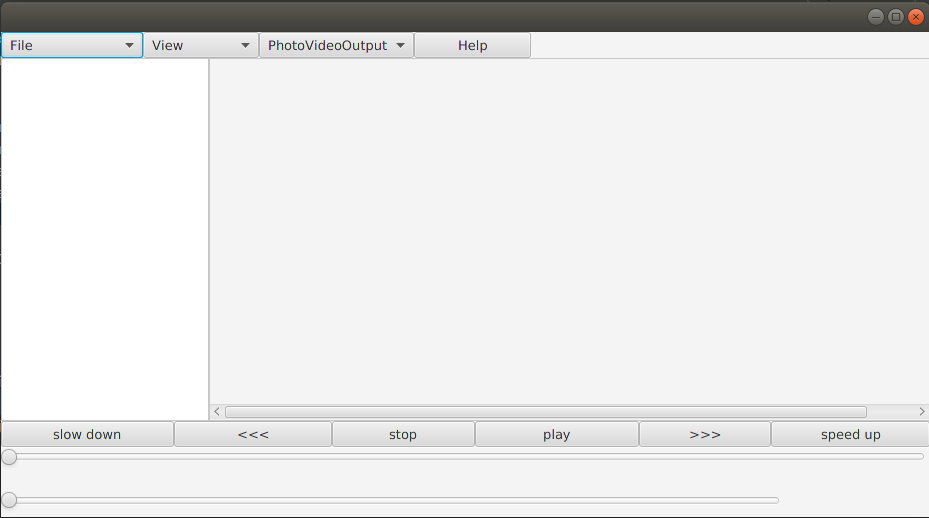
\includegraphics[scale=0.34]{main.png}
	\caption[Main toolbar]{Main toolbar}\label{fig:float19}
\end{figure}


\subsection{File}

In \verb|File| menu user could:
\begin{itemize}
\item upload new solution
\item start visualization process
\item check solution parameters 
\item clear the visualization screen  
\end{itemize}

\subsubsection{New solution}

\verb|New solution| button opens window for setting up input files. There are three types of files that has to be uploaded.\ref{fig:float20}

\begin{figure}
	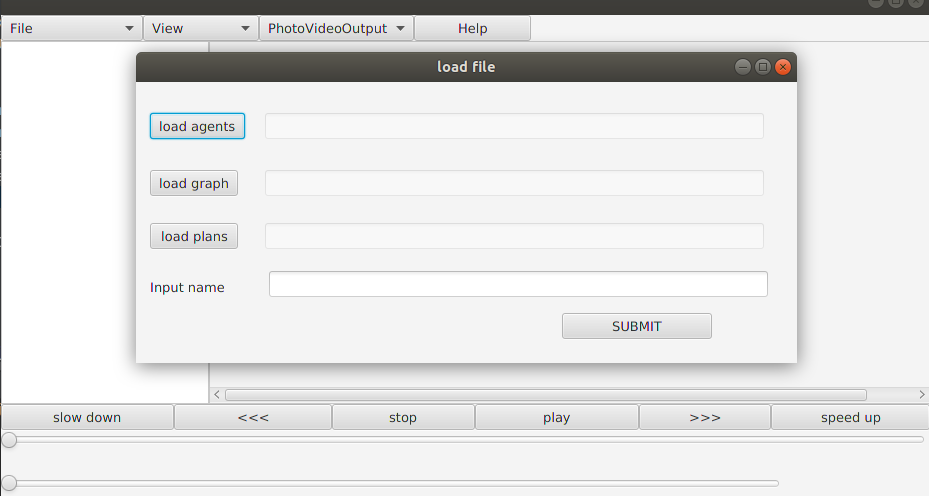
\includegraphics[scale=0.34]{loadfile.png}
	\caption[Load file]{Upload new solution dialogue}\label{fig:float20}
\end{figure}

\verb|Load agents| button opens file dialogue to set up file with agents parameters. \verb|Load graph| button opens file dialogue to set up file with graph parameters. \verb|Load plans| button opens file dialogue to set up file with agents plans. In text field user should input solution name. \verb|SUBMIT| button initiates uploading data from files and creating new solution. This new solution then appears in the uploaded solutions list(left side of main window). 

\subsubsection{Start visualization}

In order to visualize solution on the screen user should choose one in the uploaded solutions list, then click on button \verb|Start visualization|, which launches visualization.\ref{fig:float21}

\begin{figure}
	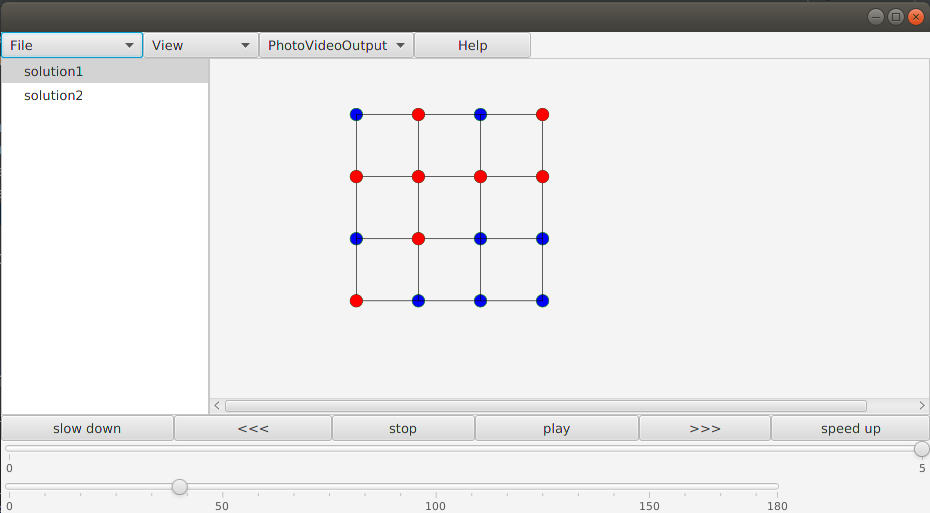
\includegraphics[scale=0.34]{solution.png}
	\caption[Start visualization]{Visualized solution}\label{fig:float21}
\end{figure}


\subsubsection{Solution parameters}

\verb|Solution parameters| button opens an information window, with such solution parameters as an amount of vertices, an amount of edges, a list of agents, etc..\ref{fig:float22} In order to open agent parameters(agent identification, start location, target location, etc),\ref{fig:float23} user should choose an agent from the list and then double-click it, as a result the agent's parameters will be shown in the right section of the window.

\begin{figure}
	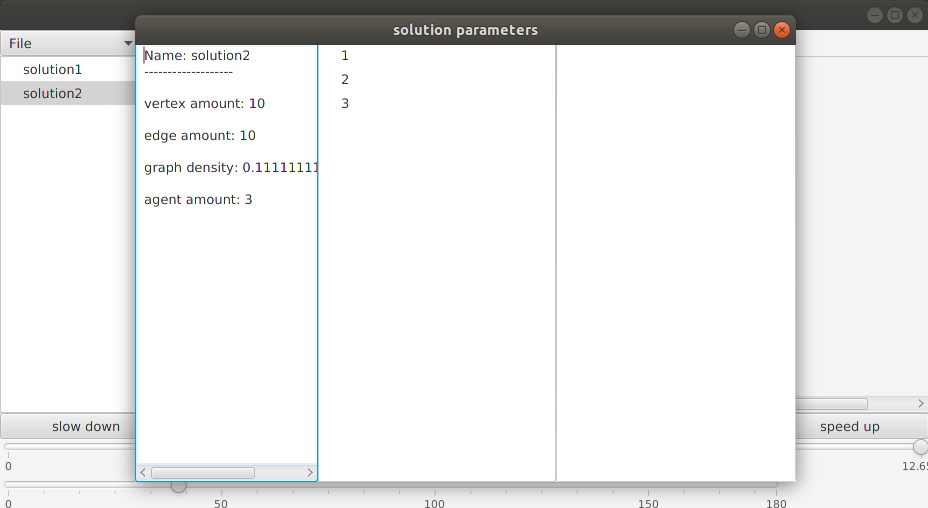
\includegraphics[scale=0.34]{solutionparameters.png}
	\caption[Start visualization]{Solution parameters}\label{fig:float22}
\end{figure}

\begin{figure}
	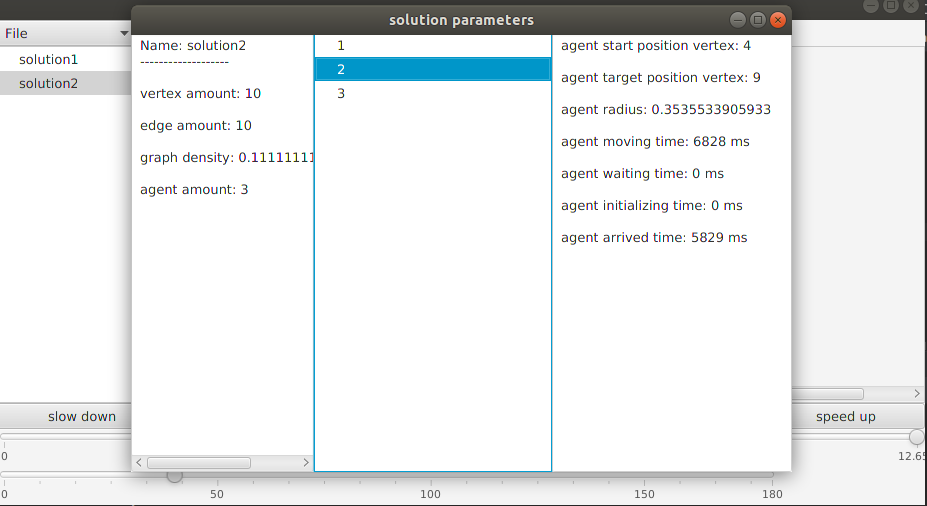
\includegraphics[scale=0.34]{agentparameters.png}
	\caption[Start visualization]{Agent parameters}\label{fig:float23}
\end{figure}



\subsubsection{Clear visualization}

\verb|Clear visualization| button removes a visualized solution from the screen.

\subsection{The visualization screen}

Graph and agent objects are displayed on the visualization screen. 

\subsubsection{Zooming}

In order to zoom in or zoom out user should put a cursor on the graph and scroll in or scroll out respectively.Zooming in and zooming out is activated by touchpad. 

\subsubsection{Marking agents}

In order to mark an agent, user should click on it. In order to unmark it user should click on it again. By default marked agent color is not set up, so user should set it up manually in Color settings.

\subsection{View}

In the view menu user could:
\begin{itemize}
\item open the single agent statistics window
\item open the double agent statistics window
\item open the color settings window
\item manipulate visibility settings
\end{itemize}


\subsubsection{Single agent statistics}

\verb|Single agent statistics| button opens window with single agent statistics interface.

\subsubsection{Double agent statistics}

\verb|Double agent statistics| button opens window with double agent statistics interface.

\subsubsection{Change color}

\verb|Change color| button opens a window with color settings interface. The window  
has several color\label{fig:float24} palettes: moving agent, waiting agent, initialized agent, arrived agent, marked agent, vertex. First yser has to define all this color palletes. Afterwards \verb|SUBMIT COLOR| button applies color settings.   

\begin{figure}
	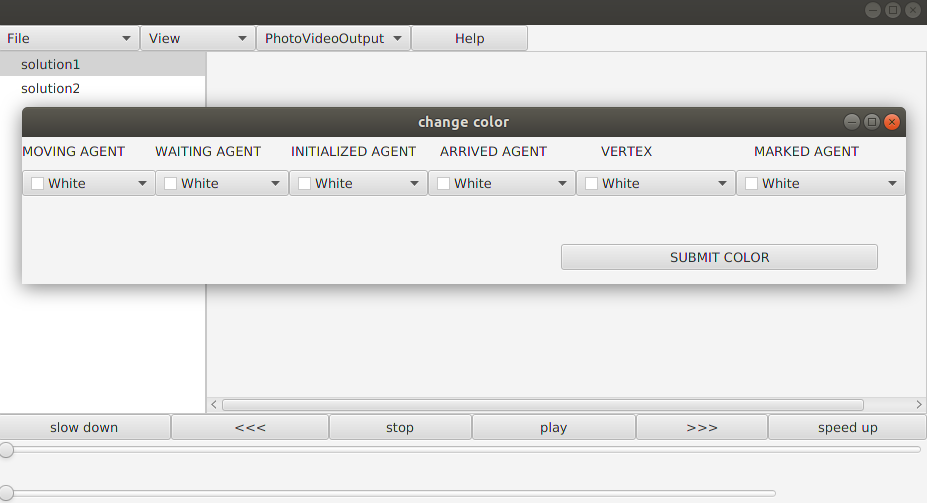
\includegraphics[scale=0.34]{solutioncolorchange.png}
	\caption[Solution color change]{Solution color change}\label{fig:float24}
\end{figure}

\subsubsection{Graph visible}

\verb|Graph visible| button changes graph visibility settings. If the graph is visible, it will be invisible, otherwise it returns to its initial visible state.\ref{fig:foat25}

\begin{figure}
	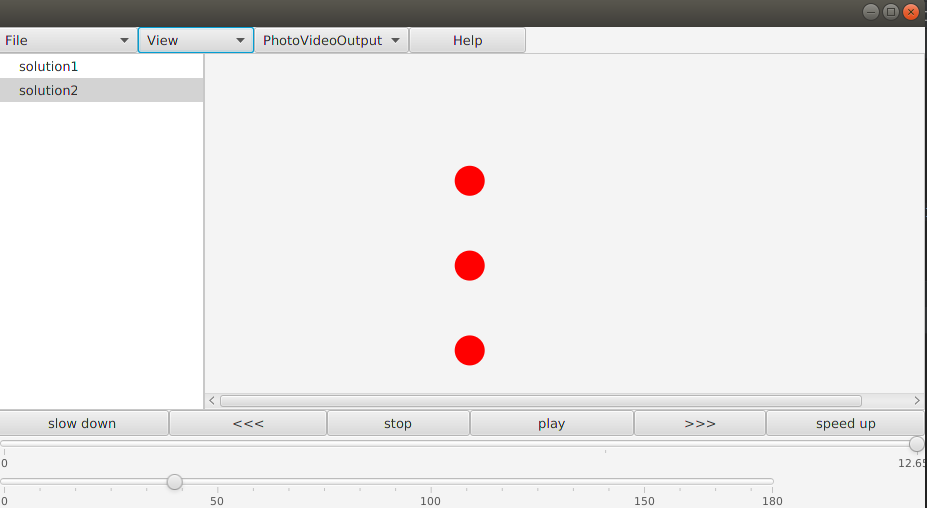
\includegraphics[scale=0.34]{not-visiblegraph.png}
	\caption[Not visible graph]{Graph is not visible}\label{fig:float25}
\end{figure}

\subsubsection{Agent visible}

\verb|Agent visible| button changes visibility of agents. It makes not marked agents invisible and it leaves marked agents visible on the screen. To return all agents back to its visibility, user should click \verb|Agent visible| button again.\ref{fig:float26}\ref{fig:float27} 

\begin{figure}
	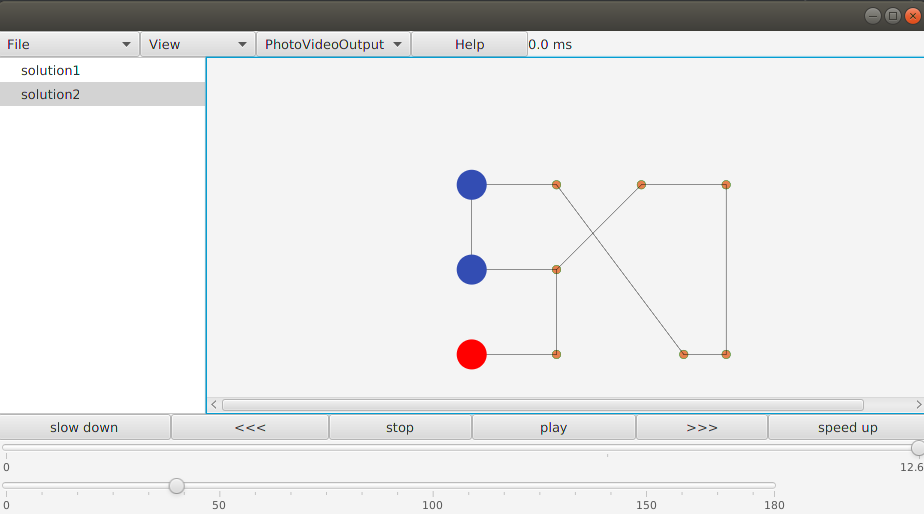
\includegraphics[scale=0.34]{markedagent.png}
	\caption[Marked agent]{Marked agents}\label{fig:float26}
\end{figure}

\begin{figure}
	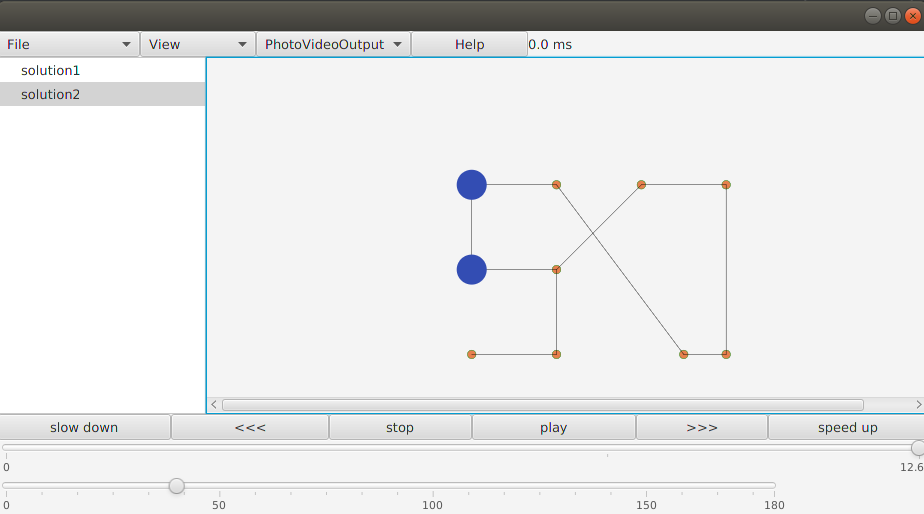
\includegraphics[scale=0.34]{unvisibleagent.png}
	\caption[Visibility agents]{Marked agents are visible, not marked agent is invisible}\label{fig:float27}
\end{figure}

\subsection{PhotoVideoOutput}

\verb|PhotoVideoOutput| menu button contains buttons that are responsible for multimedia output.

\subsubsection{Take snapshot}

\verb|Take snapshot| button creates photos of visualization screen and of single/double statistics screen, if they are opened at the moment.

\subsubsection{Start video/Stop video}

In order to begin video capture user should activate \verb|Start video| button. Video captures everything that happens on the screen. \verb|Stop video| stops video capture.

\subsubsection{VideoSettings}

In order to set resolution of video recording user should activate \verb|Video settings| button. Then input height and width parameters of video recording. Pay attention, that you should input value, which is one point lesser than monitor parameter. For instance, if your monitor resolution is 1366*768, you should input width:1365, height:767.\ref{fig:float28} 


\begin{figure}
	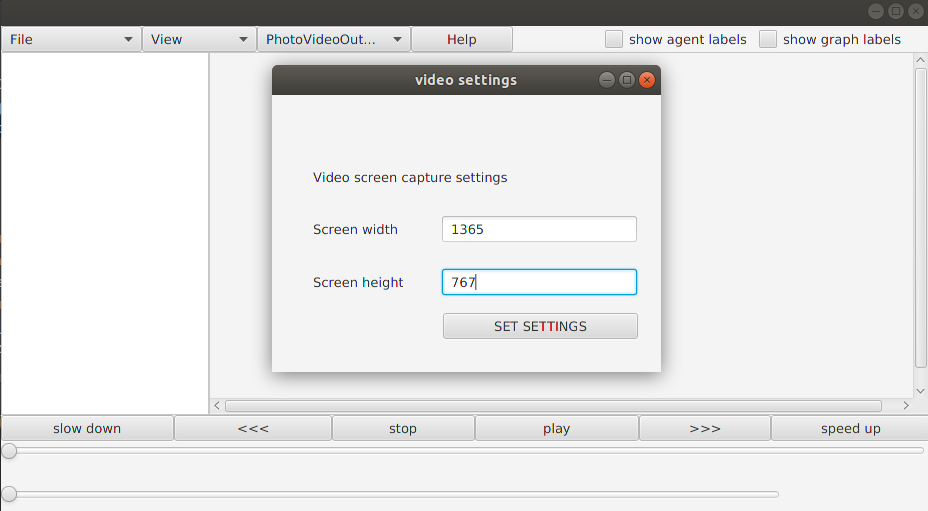
\includegraphics[scale=0.34]{VideoSettings2.png}
	\caption[Video settings]{Set width and height}\label{fig:float28}
\end{figure}


\subsection{Help}

\verb|Help| button opens the user manual.

\subsection{The visualization control panel}

The visualization control panel is an interface that manipulates the visualization process. \verb|play| button starts an animation, \verb|pause| button pauses the animation, \verb|stop| button stops the animation. When the animation is being played,  \verb|timer| appears on top of the screen and starts running. \verb|>>>| and \verb|<<<| buttons change direction of the animation, forwards and backwards respectively. To adjust speed user could use \verb|speed up| or \verb|slow down| buttons. 

Among the visualization controllers there are two sliders. The top slider controls a timeline position. By using \verb| the timeline slider| user could adjust time of the animation. The down slider controls a rotation state. User could use \verb|the rotation slider| to adjust an angle of the visualization screen.

\section{The single agent statistics window overview}

The single agent statistics window showcases statistical data, that are related to the one single agent.\ref{fig:float29} First user should input an agent index, statistical data will be shown specifically for the agent with inserted index.

The time ratio chart displays data, that are linked to the agent states: MOVING, WAITING, INTIALIZING, ARRIVED. 

\verb|Time ratio mode| menu button has two options, \verb|total time ratio| and \verb|agent time ratio|. \verb|total time ratio| activates the bar chart with the total time ratio data. \verb|agent time ratio| activates the bar chart with the time ratio data, that are relevant for the chosen agent. It is possible to display the total time ratio and the single agent time ratio at the same time, which is useful for a comparison analysis.\ref{fig:float30}

\begin{figure}
	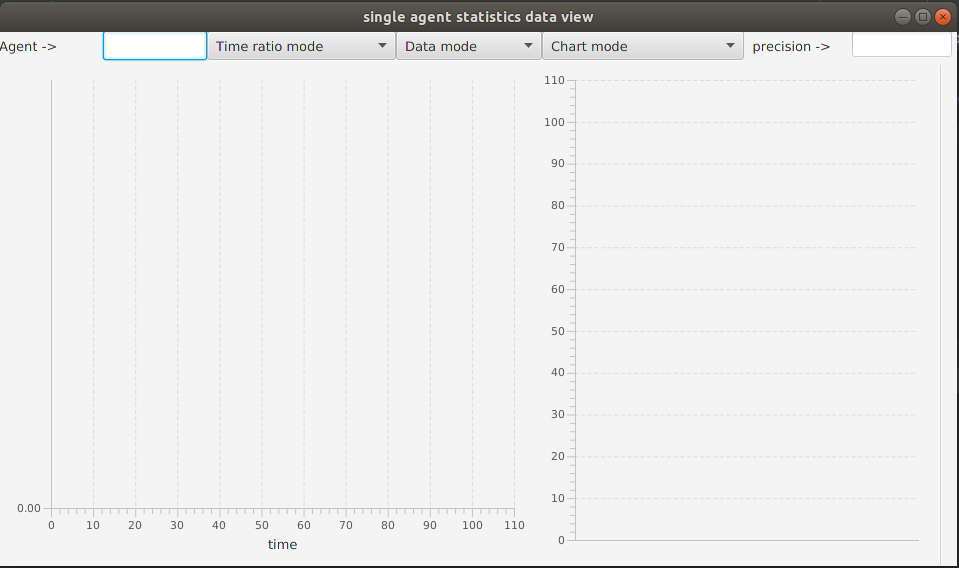
\includegraphics[scale=0.34]{SingleAgentStatistics.png}
	\caption[Single Agent Statistics]{The single agent statistics window}\label{fig:float29}
\end{figure}

\begin{figure}
	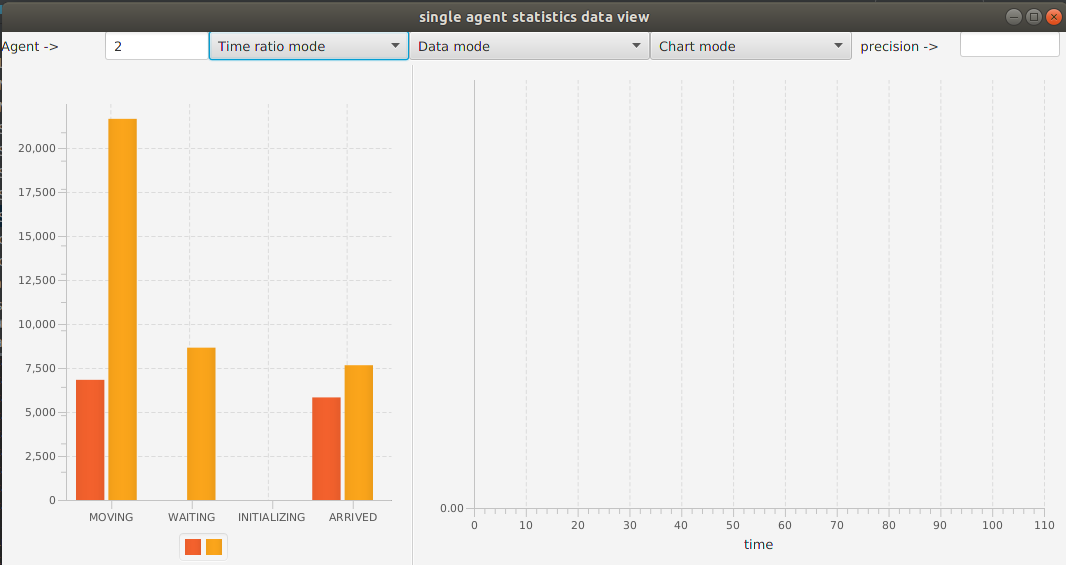
\includegraphics[scale=0.34]{ratiochart.png}
	\caption[Ratio Chart example]{Ratio Chart example}\label{fig:float30}
\end{figure}



\verb|Data mode| menu button has two options: \verb|Speed mode| and \verb|Location mode|. \verb|Speed mode| is a function that displays agent speed value at the current time of movement. \verb|Speed mode| is a function that displays agent location value at the current time of movement.

\verb|Chart mode| menu button sets up how data is going to be displayed. \verb|Real-time mode| starts displaying as animation starts playing. Data updates every second, therefore it is recommended to slow down animation speed\ref{fig:float31}. \verb|Not real time mode| displays data independently on animation playing. To set frequency rate in \verb|the precision| text field user should insert the period of milliseconds. The minimum value is 60, since the animation is displayed in Java FX standard 60 fps,  the maximum value is the total duration of the animation.\ref{fig:float32}.  

\begin{figure}
	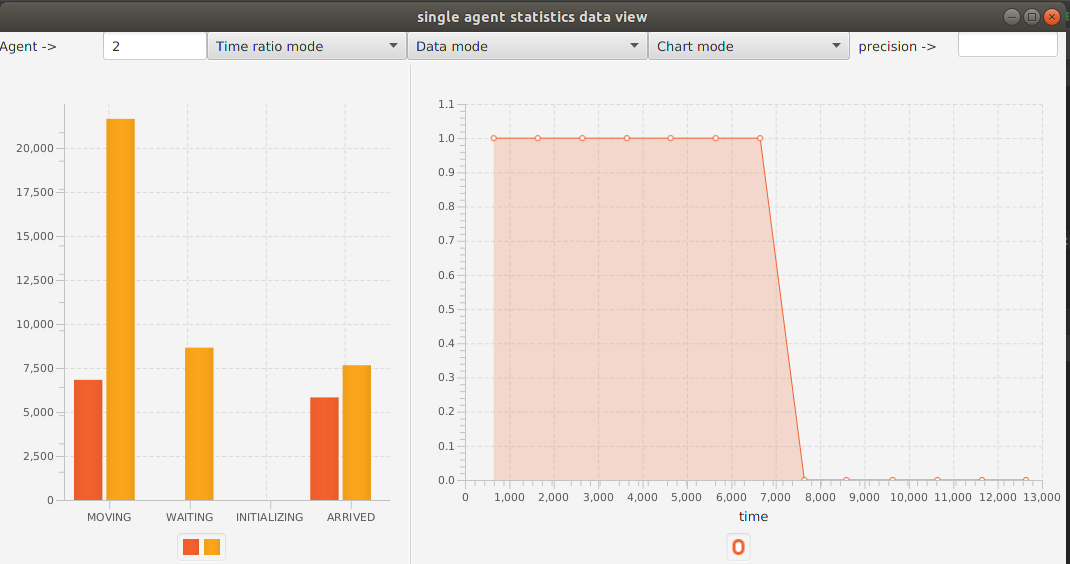
\includegraphics[scale=0.34]{onlinechart.png}
	\caption[Online chart mode]{Single agent real-time chart mode}\label{fig:float31}
\end{figure}

\begin{figure}
	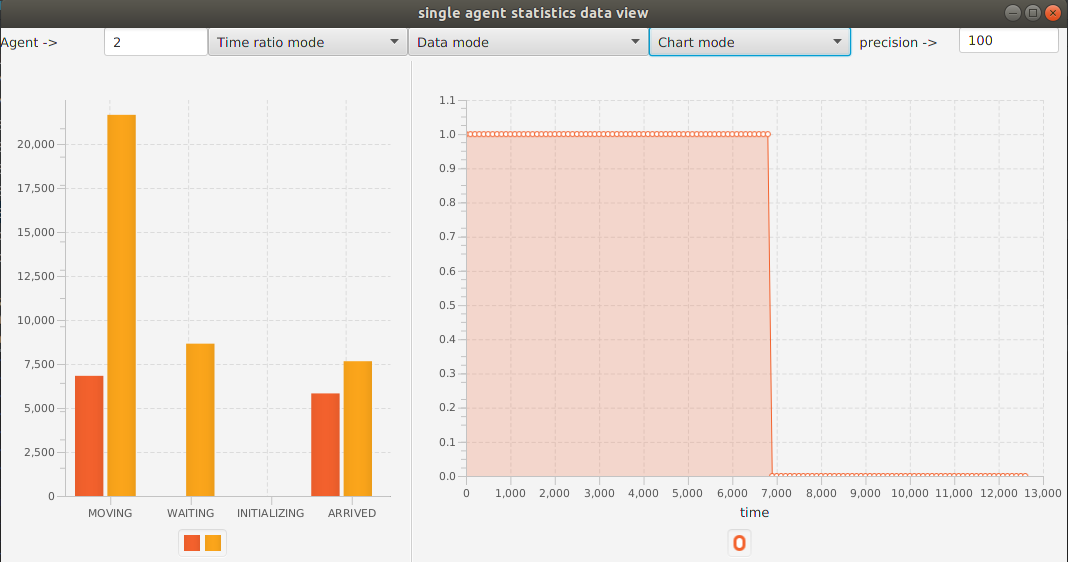
\includegraphics[scale=0.34]{not-onlinechart.png}
	\caption[Not Online chart mode]{Single agent not real-time chart mode}\label{fig:float32}
\end{figure}


\section{The double agent statistics window overview}


\begin{figure}
	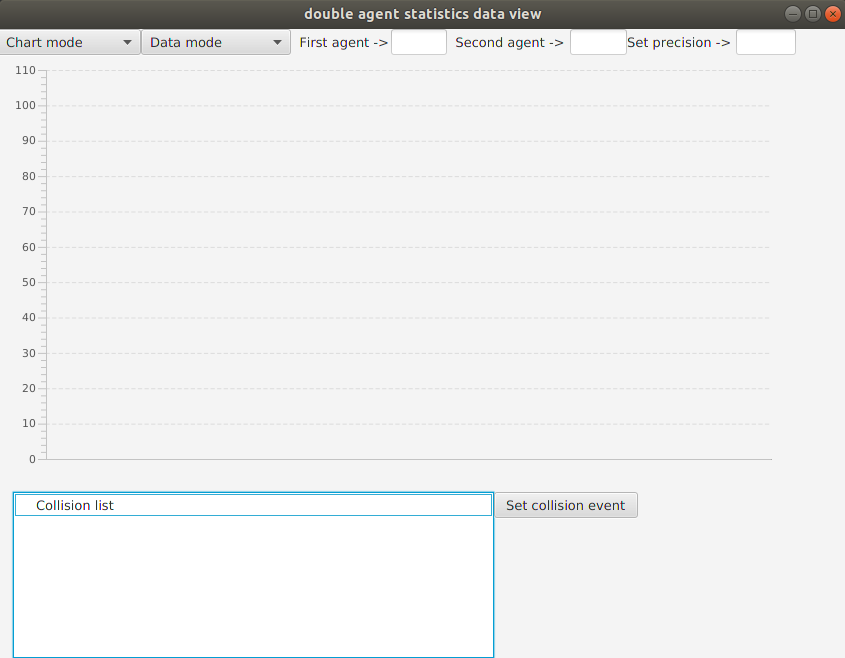
\includegraphics[scale=0.34]{DoubleAgentStatistics.png}
	\caption[Double Agent Statistics]{The double agent statistics window}\label{fig:float33}
\end{figure}

The double agent statistics window showcases statistical comparison data between two agents. User should insert two indexes, each one corresponds to its relative agent.\ref{fig:float33}

\verb|Chart mode| button menu button sets up how data is going to be displayed. It has the same options as \verb|Chart mode| button in the single agent statistics interface.\ref{fig:float34}\ref{fig:float35}

\verb|Data mode| menu button has two options. \verb|Distance mode| is a function that displays the distance between two agents at the current time of movement. \verb|Collision risk mode| is a function that displays the rate of collision risk between two agents at the current time of movement.

Collisions are displayed in \verb|Collision list|. In this list agents involved in collision event are presented as well as time of collision event. User should click on the collision event list item and click button \verb|Set collision event|. Afterwards on the visualization screen there are only selected agents left. To make all agents visible again, user should click \verb|agents visible| button.
\begin{figure}
	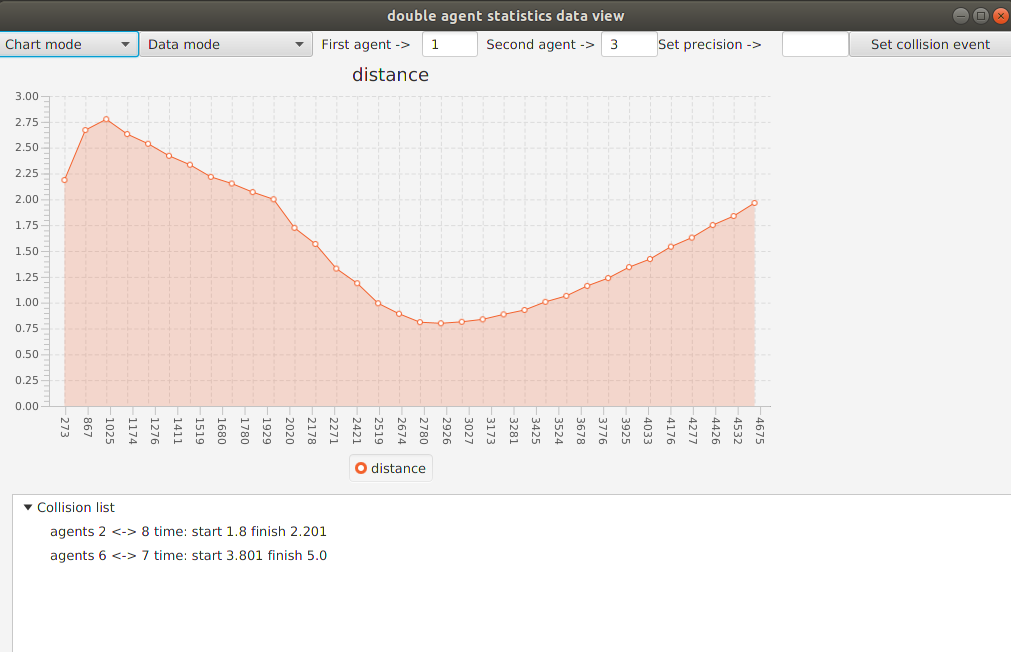
\includegraphics[scale=0.34]{onlinechart2.png}
	\caption[Online chart mode2]{Double agent real-time chart mode}\label{fig:float34}
\end{figure}

\begin{figure}
	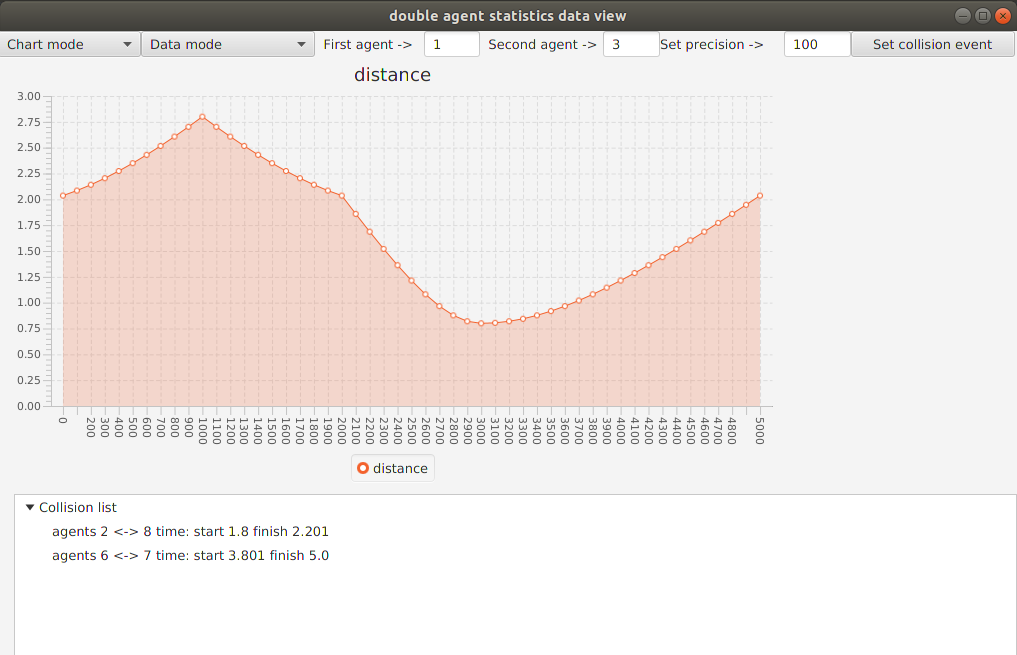
\includegraphics[scale=0.34]{not-onlinechart2.png}
	\caption[Not Online chart mode2]{Double agent not real-time chart mode}\label{fig:float35}
\end{figure}

\section{The group agent statistics window overview}

The group agent statistics window showcases statistical comparison data between a group of agents. User should insert mark agents on the main window, then by clicking \verb|set group agents| button the group is set - agent indexes appear in the list.\ref{fig:float37}

Similar to previous statistics windows \verb|Data mode| menu button has two options: \verb|Distance mode| and \verb|Collision risk mode|. \verb|Distance mode| displays average distance value within the group of agents, meanwhile \verb|Collision risk mode| displays average risk collision between agents in the group. \ref{fig:float36}

\begin{figure}
	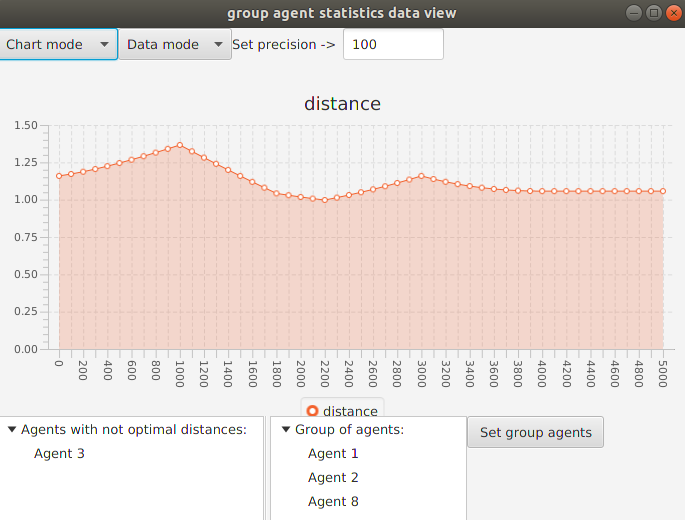
\includegraphics[scale=0.34]{GroupAgentStatisticsNotOnline.png}
	\caption[Online chart mode2]{Group agent chart statistics data}\label{fig:float36}
\end{figure}

\begin{figure}
	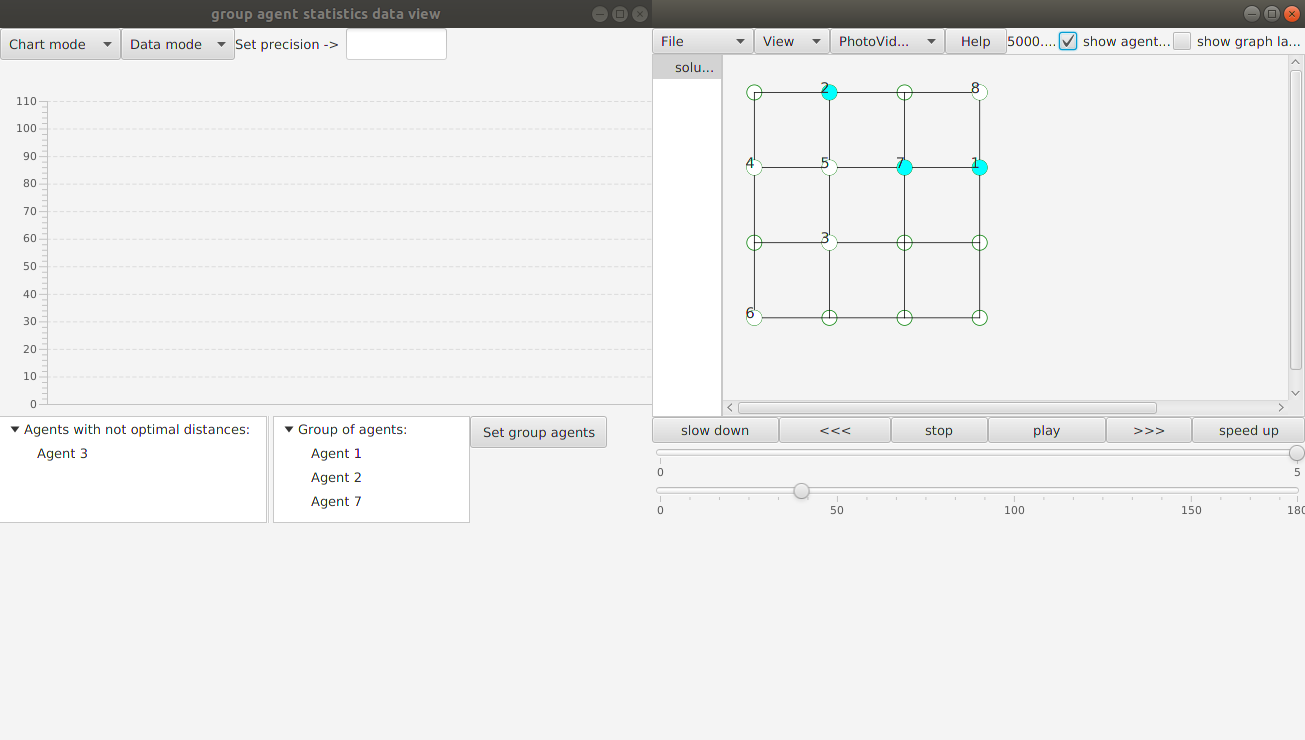
\includegraphics[scale=0.34]{GroupAgentStatisticsSettingGroup.png}
	\caption[Not Online chart mode2]{Setting up group of agents}\label{fig:float37}
\end{figure}



\chapter{Comparison analysis}

In this chapter we must convey a comparison analysis between MAPF-R visualization tool ContinuousViz and its predecessor Graphviz, which is a MAPF problem visualization tool, in order to consider their similarities and distinctions. 

\subsection{Conceptual analysis}

Graphviz is a software which is developed for visualization of MAPF problem presented in discrete time. Brief description of how it works:

\begin{description}
\item [1:]  As an input, it gets the problem provided by the user, the problem contains graph definition, initial positions of agents and the list of agent movements
\item [2:] Graphviz loads the input and calculates nodes positions in order to generate graph layout 
\item [3:] Afterwards, user sets up colors of nodes and agents
\item [4:] Finally, user navigates through the animation as with video recorder with a possibillity to record it\cite{bib_4}
\end{description}


As it can be seen, ContinuousViz follows the similar pattern.

In terms of software purpose both tools are similar. Graphviz, as well as ContinuousViz, visualizes precalculated path-finding algorithm results in order to detect redundancies of presented solution. Additionaly, they both have applications in education and presentation domains.

The main difference between Grafviz and ContinuousViz consists in time processing, i.e. while the first operates in discrete time the later operates with continuous time. In discrete time all moves are divided into groups that are characterized by the same time step, in continuous time all moves are divided into groups that are characterized by the same time interval. That changes the way the animation of the moves are approached. In Graphviz animation is played through time steps, where to adjust speed means to alter how fast time steps are changing. In ContinuousViz animation is played in real time, where to adjust speed means to alter how fast time is flowing. Timeline in Graphviz allows to jump quickly between \verb|time steps|, in ContinuousViz it allows to jump between \verb|time|. Grafviz has implemented \verb|color differentiation| in order to highlight different states of the agent, ContinuousViz disposes with identical option. Graphviz allows several animation players on single screen in order to play them simulteniously, meanwhile ContinuousViz does not have that option. It has been decided that several animations at the same time on single screen has a potential to rise the complexity level of visual analysis. 

Graphviz enables modification of graph form, meanwhile ContinuousViz strictly follows graph predefinition derived from input data, i.e. vertex placement is predefined by coordinates values. This restriction is reasoned by the fact that MAPF-R graph replicates real world space structure.


\subsection{Technological analysis}

In terms of technology Graphviz uses Qt cross-platform application and GUI framework, as a programming language it uses C++. ContinuousViz uses JavaFX GUI framework. as a programming language it uses Java. As for video capture, Graphviz, as well as ContinuousViz, uses FFmpeg video library. In terms of operation systems, both Graphviz and ContinuousViz are compatible with Windows, Linux and MAC OS. Graphviz supports extensibility of its functions and, similarly, ContinuousViz does that as well. Both Graphviz and ContinuousViz have modular architecture as their component parts represent interchangable modules. As far as licensing is concerned, they both are open-source software.

\subsection{Comparison summary}

\begin{table}[h]\label{fig:float100}
\centering
\caption[Comparison analysis summary]{Comparison analysis summary}
\begin{tabular}{|l|l|l|}\hline
Parameter		& ContinuousViz & Graphviz
\tabularnewline \hline \hline
time & continuous time & discrete time
\tabularnewline \hline \hline
programming language & Java & C++
\tabularnewline \hline \hline
GUI tool & Java FX & QT
\tabularnewline \hline 
multiplatfom & yes & yes
\tabularnewline \hline
open-source & yes & yes
\tabularnewline \hline
collision detection capability & yes & yes
\tabularnewline \hline
color differentiation capability & yes & yes
\tabularnewline \hline
vertex position change capability & no & yes 
\tabularnewline \hline
video record capability & yes & yes
\tabularnewline \hline
photo record capability & yes & yes
\tabularnewline \hline
save current configuration capability & no & yes
\tabularnewline \hline 
\end{tabular}
\end{table}


To sum all up\ref{fig:float100}, it can be said, that Graphviz has a major impact on ContinuousViz in terms of an inspiration and ideas. Some functionality design elements of ContinuousViz, for instance video player type interface, has been derived from Graphviz. However, ContinuousViz differs in a sense of time processing, subsequently design interface has to be adapted with real time movement.


\chapter{Analysis of MAPF-R visualization tool ContinuousViz economic impact on logistics}

In this chapter we will analyze economic potential of the visualization tool in logistic domains where MAPF-R is used as an underlying concept for navigating robotic manipulators.

\section{Industry 4.0}

In the beginning, it should be pointed out that visualization tool will be economically assessed  within the context of Industy 4.0. paradigm change, which is based largely on use of automated tools.\ref{fig:float38}
 
\begin{figure}
	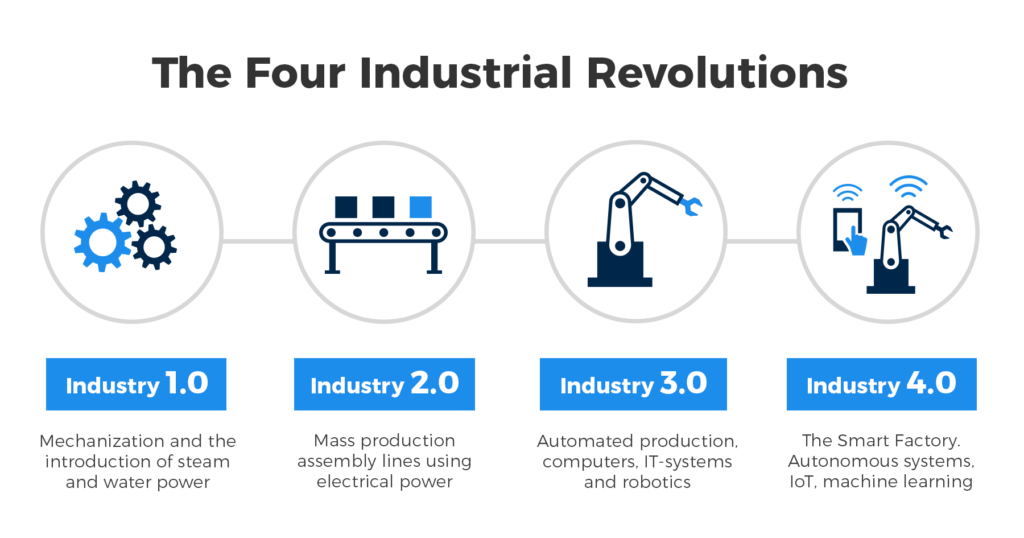
\includegraphics[scale=0.4]{SE_artikkeli_kuva_SmartIndustry_v02-1024x538.png}
	\caption[History of industrial revolutions]{History of industrial revolutions}\label{fig:float38}
\end{figure} 

Industry 4.0. is a collective term for technologies and concepts of value chain organization \ref{fig:float39}.Industry 4.0. represents such domains as advanced robotics, industrial internet, big data and analytics. Industry 4.0. is a product of the upcoming fourth industrial revolution. If the third industrial revolution had everything to do with the rise of computers, computer networks(WAN, LAN, ... ) and connectivity, in the fourth industrial revolution it is not just about the Internet and the client-server architecture, it is about merging digital and physical environments. The key objectives of Industry 4.0. is information and services. The main goals of Industry 4.0. are automation and data exchange, manufacturing process improvement and production optimization, cutomer orientation. Those goals must be achieved by blending virtual and real world together, creating cyber-physical systems(CPS).


\begin{figure}[H]
	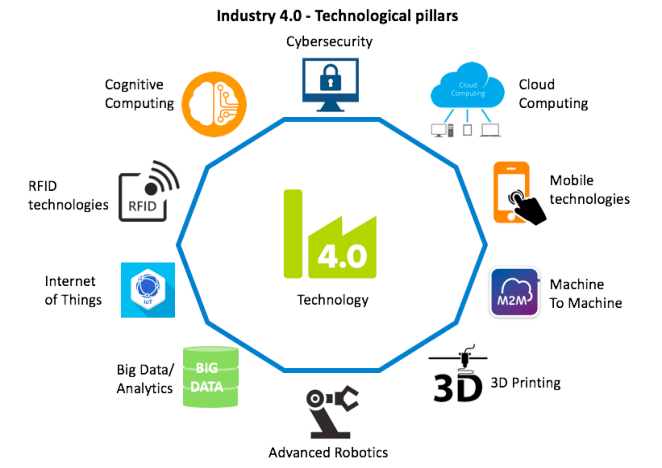
\includegraphics[scale=0.4]{Technologies-for-industry-40.png}
	\caption[Industry 4.0 technologies]{Industry 4.0. main technologies}\label{fig:float39}
\end{figure}%change float index 

In terms of technologies, the main difference between Industry 4.0 and its predecessors lies in the structure: instead of centralised structures, it implements schemes in which autonomous agents interact in decentralised architectures. The process of decision-making implements such technologies as Cloud Computing, Big Data, Internet of Things. As a matter of fact, decentralised intelligence facilitates creation of smart objects networking and independent process management. Industry 4.0. includes horizontal integration across networks, that enables internal communication, and the vertical integration of a production inside the production plant, that facilitates adaptable manufacturing systems.

Industry 4.0 can be characterized by following features:
\begin{description}
\item[Virtualization] companies have a possibility to observe physical processes, by linking sensor data to simulation data.
\item[Interoperability] All systems in and out of company are interconnected.
\item[Autonomization] In Industry 4.0 machines and algorithmns are enabled to make decisions and learn autonomously, which minimize human-machine interaction.
\item[Real-Time availability] Data is collected and analyzed in real time. The state of the plant is being scrutinized and tracked permanently.
\item[Flexibility] Due to the high customer demands, production process must become more adaptive to constantly changing production environment. 
\item[Service orientation] The services of the company can be offered internally and externally, i.e. the services can be utilized by other participants.
\item[Energy efficiency] Due to climate change it is crucial for industries to utilize carbon-neutral technologies in manufacturing. In addition, utilization of renewable energies is more financially attractive.
\end{description}


\subsection{Industry 4.0 fundamental technologies/concepts}

Main technological concepts of Industry 4.0 can be divided into four major categories: cyber-physical systems, Internet-of-Things, Smart Data and Smart Factory. 

\subsubsection{Cyber-Physical systems}

It must be noted, that  Cyber-Physical Systems(CPS) is considered to be the key element of Industry 4.0., as they facilitate the confluence of physical and virtual spaces, integrating computational and communication processes in interaction with physical processes. CPS are physical systems, whose operations are being monitored and controlled by communicating and computing system. A relevant instance of CPS can be represented by intelligent manufacturing lines, in which single machine can carry out a variety of procedures communicating with other components. CPS consists of a set of networked elements, that include sensors, control processing units, actuators, communication devices. Intelligent CPS has a potential to spur innovation in such industries as aerospace, infrastructure, transportation, energy, chemical domains and logistics services. CPS has an ability to cover all the stages of production processes, starting from shop floor to logistics networks, consequently shorten the production cycle. 

Cyber-Physical Systems represent such technologies as embedded technologies, Component machine health, Smart analytics, Remote visualization for human, Multidimensional data correlation, Degradation and perfomance prediction, etc.

\subsubsection{Internet of Things}

Internet of things(IoT) is a system where physical devices are bonded with embedded electronics(RFId tags, senosrs, etc) and they are connected to the Internet. In the context of IoT physical objects are integrated into the information network, which enables them to become active participants in business processes. Via the internets physical device can message its status, its environmental surroundings, maintenance schedule, production processes, etc. IoS facilitates service vendors to offer  services via the internet. It consists of participants, an infrastructure for services, business models and the services themselves.  

IoT includes following technologies: sensors, mobile technologies, RFID, Rectivity sensors, hardware interfaces, smart objects, smart networks, data acquisition systems, which connect the machines to suppliers, network of devices, human-computer cooperation, etc. 

\subsubsection{Smart data}

In the context of Industry 4.0 a plant will be producing a huge amount of data that needs to be stored, processed and \verb|intelligently| analyzed. Big data handled by innovative methods and cloud computing have a potential to create new ways to advantage information.

Smart dat includes following technologies big data, electronic documents, analyzing and storing data, simulation models, sensor data, production status, energy consumption behavior, etc. 

\subsubsection{Smart factory}

Inside the factory of Industry 4.0 new technologies will be used, alongside new materials and new ways to handle production data. Smart factory consists of following subcategories: Smart product, smart logistics, 3D visualization, Smart Manufacturing process, Modularization of processes and products, decentralized intelligence, 3D-printing, efficient manufacturing, self optimization and reconfiguration machines, etc. \cite{bib_5}  


\section{Visualization in Industry 4.0}

In this section different visualization techniques, that is being used in Industry 4.0, will be described. In smart manufacturing \verb|data analysis| supports decision-making processes at all stages of production lifecycle. In the context of large and complex data sets, visualization has become a predominant tool, which is able to combine machine intelligence and human intelligence in order to gain insights from data, that could lead to efficiency improvement and process optimization.\ref{fig:float40}

Visualizaion techniques can be divided by the concepts of \verb|replacement| and \verb|creation|. The replacement concept implements visualization tools in order to simulate physical reality in virtual space, whereas creation concept uses visualization tools as navigation during the product creation process. 

\begin{figure}
	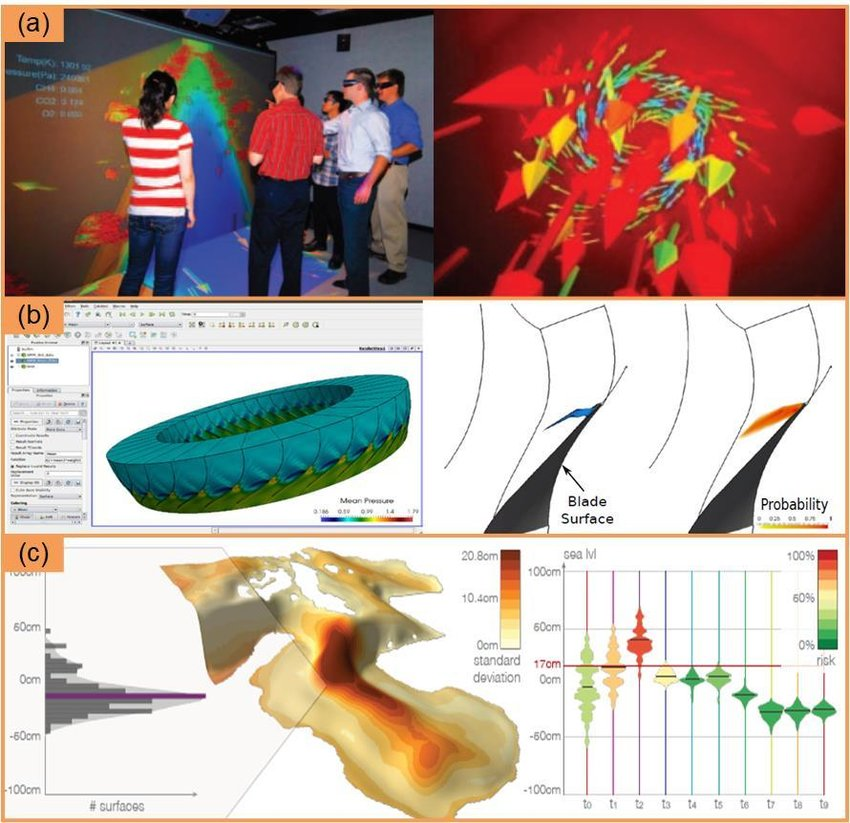
\includegraphics[scale=0.6]{VisualizationInIndustry.jpg}
	\caption[Application cases of scientific visualization in industry manufacturing. (a) Steelmaking furnace internal environment visualization; (b) Jet engine internal environment visualization; (c) Oil exploration external environment visualization.]{Application cases of scientific visualization in industry manufacturing. (a) Steelmaking furnace internal environment visualization; (b) Jet engine internal environment visualization; (c) Oil exploration external environment visualization.}\label{fig:float40}
\end{figure} 

\subsection{Visualization replacement concept}

As far as replacement is concerned various kinds of immersive visual technologies are being utilized: Virtual reality(VR), Augmented reality(AR), Mixed reality(MR)\ref{fig:float39}. Such technologies enable to simulate dangerous and complex work scenarios in a computer generated environment, where human operators can be taught new skills harmlessly and informatively. AR technologies can function as a graphic interface, that sends messages and instructions to human operator. As an example, worker can efficiently master assemble order by reading instructions on AR glasses. One major direction in the replacement concept is a scientific visualization. It aims to model and analyze industrial environment, for instance the flame inside a complex gas combustion system, in order to deepen the understanding of complex systems. With scientific visualization it is possible to gain almost intuitive perception of complex industrial system by human operator.

\begin{figure}
	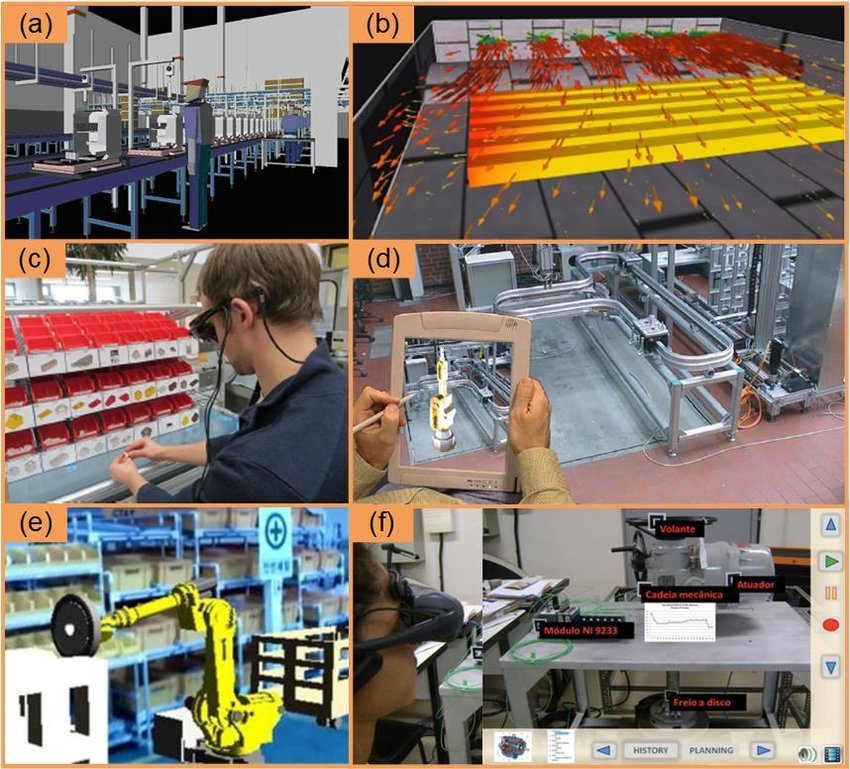
\includegraphics[scale=0.6]{VisualizationVR.jpg}
	\caption[Application cases of VR, AR and MR in industry manufacturing. (a) VR assembly factory; (b) VR furnace hot gases escaping; (c) An assembly worker wearing AR glasses; (d) AR supported production line modeling; (e) MR workshop environment; (f) MR equipment interface.]{Application cases of VR, AR and MR in industry manufacturing. (a) VR assembly factory; (b) VR furnace hot gases escaping; (c) An assembly worker wearing AR glasses; (d) AR supported production line modeling; (e) MR workshop environment; (f) MR equipment interface.}\label{fig:float41}
\end{figure} 

\subsection{Visualization creation concept}

Visualization within the creation concept is being used during the production process of new values for both makers and consumers. The beginning of production cycle is a product \verb|design phase|, which defines appearance, function and perfomance of a product based on market demand and creative thinking. In this phase visualization can be applicable in regards to determination of design constraints, concerning prototype appearance and function. In the next \verb|production phase|, during which prototype transforms into physical object, visualization is used to fulfill the main goal of this phase - to maximaze production efficiency. Human operators are provided with real-time data visualization to control and monitor production process. It also facilitates production managers to collect and analyze non-real-time historical data in order to innovate production process, therefore making it more efficient. The next phase is \verb|testing phase|, which includes confirming if final product satisfies predefined requirements.\ref{fig:float42} Usually production tests generate a massive amount of data sets, which makes data analysis extremely difficult to convey. With the help of visualization tools test engineers can make a subsets out of multivariate parameter space, for instance injection rates of car engines, and test those specific parameters. Visualization also enables test products by simulating different physical environments, for example water waves or light condition, to test product behaviour pattern in those environments.\cite{bib_6}

\begin{figure}
	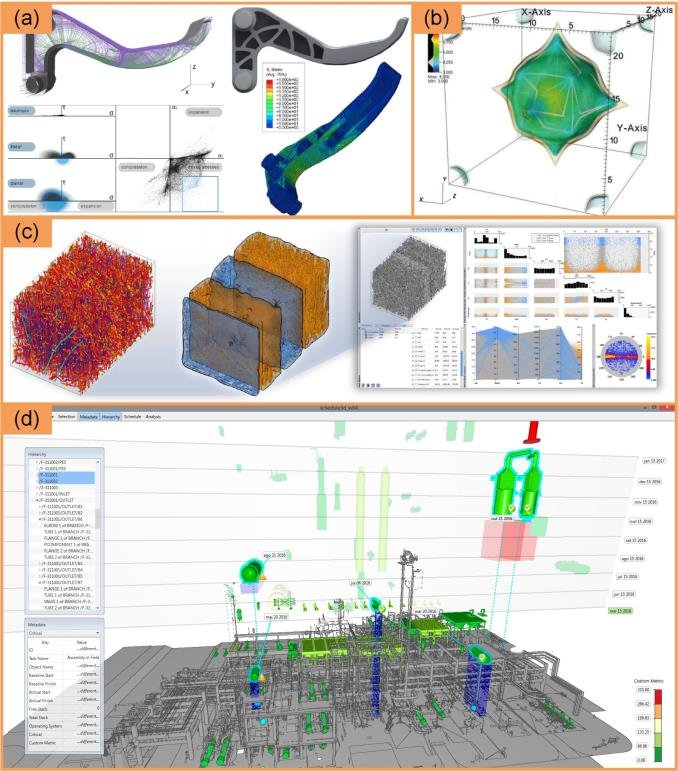
\includegraphics[scale=0.7]{VisualizationStructuralDesign.jpg}
	\caption[Visualizations for design phase: (a) Structural design of product; (c) Material characteristics analysis; (d) Production environment design.]{Visualizations for design phase: (a) Structural design of product; (c) Material characteristics analysis; (d) Production environment design.}\label{fig:float42}
\end{figure} 



\section{Smart Logistics}

As far as logistics domain is concerned, it has to adapt its business processes to Industry 4.0. requirements. Smart Logistics is a term, which decribes the combination of logistics updated with CPS. The following technological systems will serve as the  structural elements of Smart Logistics: Resource Planning, Warehouse Management Systems, Intelligent Transportation Systems and Information Security\ref{fig:float43}. Warehouse Management Systems(WMS) has a major role in Smart Logistics, as it is a vital part of a supply chain, connecting production process and delivery. Therefore, Smart Warehouses, where intelligent warehouse management system select and adjust docking slot in accordance with transport arrival time, could drastically increase level of customer services. At this point MAPF-R visualization tool may be used as an information representation system within Warehouse Management System.\cite{bib_7}

\begin{figure}
	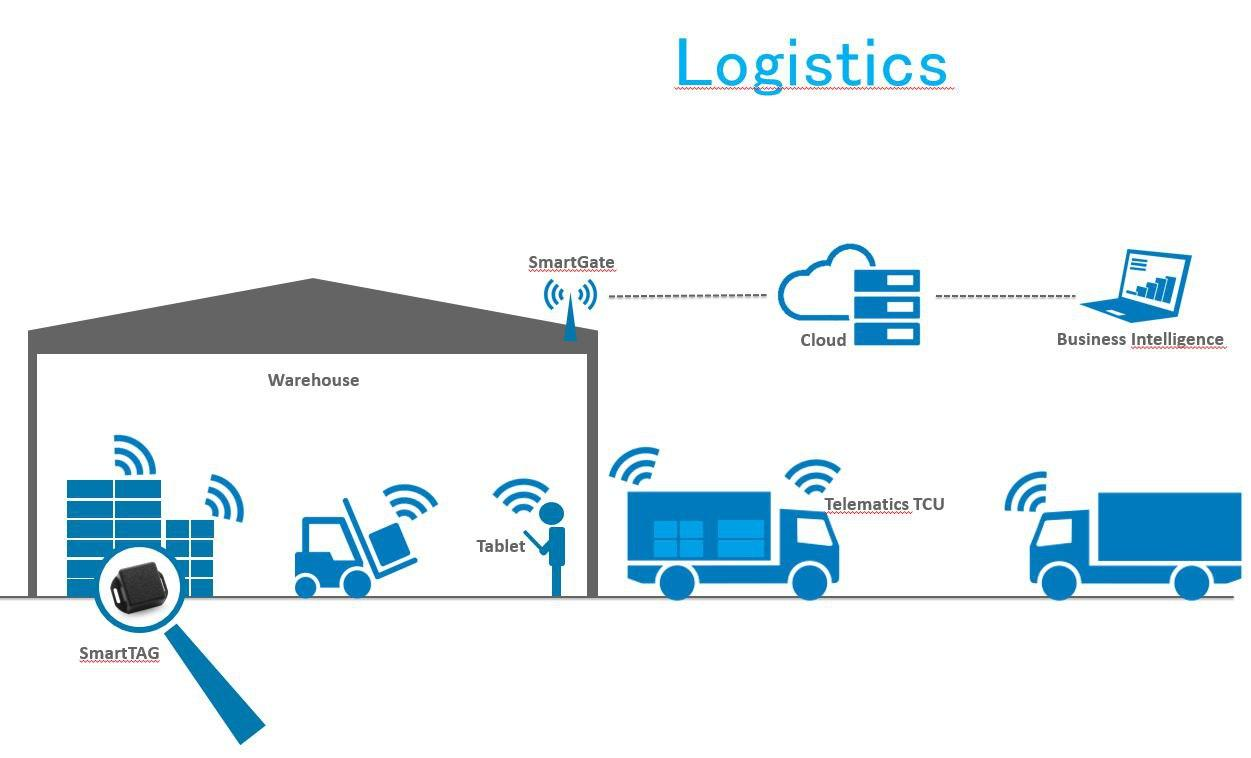
\includegraphics[scale=0.4]{smartlogistics.jpg}
	\caption[Smart logistics]{Smart logistics concept}\label{fig:float43}
\end{figure}


\subsection{Amazon warehouse automation experience}

In order to analyze an economic impact of robotic manipulators on logistics, it has been decided to take Amazon experience of implementing warehouse automation as a basis for this analysis.\ref{fig:float43}

Online retail giant Amazon has updated its warehouses with robotic manipulators, which led to dramatic increase in logistics system productivity. In the year 2012, Amazon acquired Kiva Systems, the company that makes robots, for 775\$ million, and since 2014 more than 100.000 of the machines in 25 of its 149 warehouses worldwide have been deployed. When item is delivered to warehouse, it is being given location at the warehouse and scanned, so the computer knows where item is located. When item is ordered warehouse bot picks it up from its location and transports it. 


\begin{figure}
	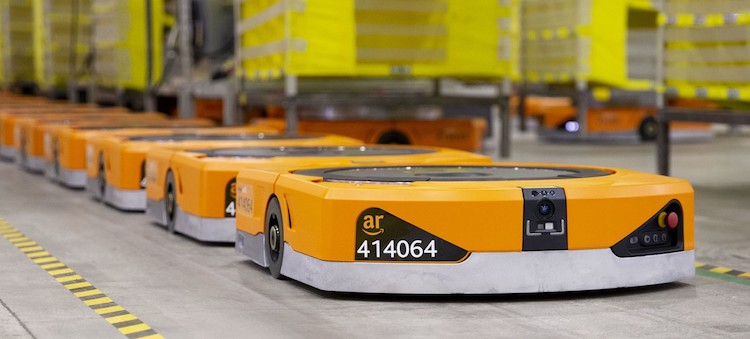
\includegraphics[scale=0.3]{Amazon/3.jpg}
	\caption[Amazon warehouse bots(a)]{Amazon warehouse bots(a)}\label{fig:float44}
\end{figure}

When Amazon fulfillment centers has been introduced to new sorting system - Pegasus, that implements bots to sort orders. It allowed Amazon to increase sorting accuracy up to 50 percent, i.e. introduction of robotic manipulators has increased the level of customer services by cutting down the risk of mis-sorted goods. Furthermore, introduction of CartonWrap machines, that are capable to box 600-700 boxes per hour(5 times the rate of manual human packer), will definitely shorten delivery time. In fact, as was estimated in 2016 by Deutsche Bank, delivery "click to ship" cycle, which is the time it takes to pick a product from the stacks, pack it and ship it, was approximately from 60 to 75 minutes when human workers manually handled the process, then robots have been introduced and the same job could be accomplished in 15 minutes. Considering Amazon experience it can be seen that automation of warehouses is vital as it leads to higher customer service level.\ref{fig:float45}\ref{fig:float46}
%(ref: Bussiness insider in Telegram channel)
\begin{figure}
	\includegraphics[scale=0.3]{Amazon/2.png}
	\caption[Amazon warehouse bots(b)]{Amazon warehouse bots(b)}\label{fig:float45}
\end{figure}


Although automation of Amazon warehouses has a vast majority of benefits, concern is being made that warehouse workers could be negatively affected by that. In fact, as Amazon states, the machines are capable to replace at least 24 jobs at each location they are installed. If they are installed in Amazon's 55 US fulfillment centers, they could replace 1.300 total workers. In order to solve workforce shortage, it could be possible to re-purpose or re-educate workers. For instance, it is possible to reallocate jobs away from warehouse workers towards delivery couriers. By the moment of year 2019, Amazon have implemented robotic machines which are needed of human assistance.\cite{bib_8}

\begin{figure}
	\includegraphics[scale=0.3]{Amazon/4.png}
	\caption[Amazon warehouse bots(c)]{Amazon warehouse bots(c)}\label{fig:float46}
\end{figure}


\subsection{MAPF-R visualization tool practical applications in warehouse management}


The distinction should be made between the shop floor and the higher management level in terms of usage of MAPF-R visualization tool. A shop floor is the area of a factory, machine shop, etc. where people work on machines, or the space in a retail establishment where goods are sold to consumers. The term shop floor is in contrast to office, where higher management is being handled. The difference of their main directives influences directly the way how MAPF-R visualization tool will be accustomed. In the shop floor more practical and mundain tasks are being solved, thus visualization tool will be used as a monitor displaying the situation in real-time. 

On the contrary higher management handles more strategic oriented tasks, which implies the function of visualization tool as an analytical instrument, storing and aggregating the historical data. MAPF-R visualization tool could be implemented as a part of Enterprise Resource Planning(ERP). By visualizing data set, management professionals will be able to indentify systematic errors, inefficient patterns, deeper structural problems with scheduling. Overall, that has a potential to create an opportunity for optimizing business processes.

In order to evaluate how MAPF-R visualization tool affects shop floor processes, we should model an environment, in which it will be operating. Automated warehouses combine various kinds of Cyber-physical systems(CPS), for instance, intelligent robots and autonomous vehicles. The main function of such systems in warehouse is to fulfill the inventory replenishment, storage and delivery requests. Those systems require collaborative behavior to handle effectively distribution of goods, as a result, the need of communication and real-time feedback is increasing. Therefore, CPS are \verb|producers| of a vast amount of visualized content. The warehouse manager, system engineer and warehouse staff are \verb|consumers| of this visualized content. They monitor functioning of CPS in order to control if the main warehouse Key Production Indicators(KPI) are being accomplished without any conflicts. Following KPIs are being considered: perfomance, safety, sustainability, knowledge reusability.\cite{bib_9}

The most common usage of robotic manipulators in warehouses is delivery bots, whose function is to move ordered packages from storage to its target segment in warehouse. Given smart warehouse, equipped with robotic manipulators, human operators monitoring the system and providing technical help in case of complex situations, visualization tool will function as a bridge between human and machine. Human operator monitors the progress of production and solves problems if an \verb|actual| situation deviates from a \verb|scheduled| situation. For instance, if ordered package has not reached its destination, visualization tool will demonstrate where error has occured. The next type of problem will be occurance of traffic congestion, the situation where great amount of bots jam up and get stuck en route, which slows down the package delivery process. Visualization tool also enables operator to control such problematic situations by demonstrating a congestion segment.

Regardless to all the benefits, that automation delivers, there is certain increase in complexity of overall production process. The level of sophistication required will substantially increase, throughout the IoT and the degree of specialization of human resources, i.e. computational and analytical skills will be a necessity among human operators. MAPF-R visualization tool has a potential to simplify the perception of information by visualizing complex situations, consequently making job position more acceptable for candidates.


\section{Economic assessment summary}

In this section we sum up key points of MAPF-R visualization tool ContinuousViz economic benefits
on Smart Logistics. Influence area has been divided into three domains: shop floor, top management and customer.

\begin{table}[h]\label{fig:float101}
\centering
\caption[Economic assessment summary]{Economic assessment summary}
\begin{tabular}{|l|l|}\hline
Domain		& Influence		
\tabularnewline \hline \hline
Shop floor		&• More	precise goods redistribution system
\tabularnewline 
\newline 	&• Faster actual problem detection system
\tabularnewline 
\newline 	&• More accessible problem representation for workers
\tabularnewline \hline
Top management	&•	More precise strategic planning \tabularnewline 
\newline	&• Systematic mistakes detection system	   
\tabularnewline 
\newline 	&•	Detection of weak scheduling patterns
\tabularnewline 
\newline 	&•	Great presentational tool
\tabularnewline \hline
Customer		&•	Higher satisfactory level	
\tabularnewline 
\newline 	&•	Higher customer service results in higher customer loyalty
\tabularnewline 
\newline 	&•	Customer loyalty results in higher probability of repeatable orders
\tabularnewline\hline 
\end{tabular}
\end{table}

According to this table\ref{fig:float101}, application of MAPF-R visualization tool ContinuousViz in logistics domain has a potential to be highly beneficial for all business process participants.

In a technological processes perspective it must be pointed out, that the Smart Logistics goal is not to replace humans in their works, but to avoid inaccuracies and to have faster processes where the information can be shared effortless and in real time. It will be always needed to involve people monitoring the processes and taking control of any system failure.  As a matter of fact, introduction of robotic manipulators to Amazon warehouses created a wide range of job opportunities, such as bots operators, technicians and engineers. Overall, the highest level of business process effectivity is possible to achieve solely by creating symbyosis between humans and machines, and that is where proper visualization tools can be sufficient.



\begin{conclusion}
	
Within the context of this thesis we have studied theoretical basis of MAPF-R problem and prospects of its visual analysis. As a result, we have concluded that  visualization tool of MAPF-R problem is a necessassity in order to examine it properly.

The main outcome of this thesis is the application called ContinuousViz. It has been designed, developed and successfully implemented. It operates according to its purpose - to visualize and detect weak points of the MAPF-R problem solution.  However, there are plenty of features that could expand its functionality. Potentially, it could visualize more complex graph structure, that includes several thousands of vertices and agents. In terms of analytics, ContinuousViz could potentially be merged with an AI, which facilitates data analysis with higher level of peculiarity. 

In addition, economic influence of MAPF-R visualization tool ContinuousViz on logistics domain has been studied. It has been concluded, that ContinuousViz has a broad spectrum of usage in logistics and a capability of improving the whole domain.

From a personal perspective, I would conclude, that during the process of writing this thesis and developing MAPF-R visualization tool ContinuousViz, I have become deeply interested in robototechnique in general and in motion-planning algorithms in particular. I have decided to proceed with my research work as well as with development of technological instruments in this area.

\end{conclusion}

\bibliographystyle{csn690}
\bibliography{mybibliographyfile}

\begin{thebibliography}{10}

\bibitem{bib_1}
G. Sharon, R. Stern, A. Felner, N.R. Sturtevant \textit{Conflict-based search for optimal multi-agent pathfinding.} [online]. [cit. 2020-05-05]. Available at: \url{https://www.sciencedirect.com/science/article/pii/S0004370214001386}

\bibitem{bib_2}
A. Andreychuk, K. Yakovlev, D. Atzmon, R. Stern \textit{Multi-Agent Pathfinding with Continuous Time} [online]. [cit. 2020-05-09]. Available at: \url{https://www.ijcai.org/Proceedings/2019/6}

\bibitem{bib_3}
T. Landesberger, A. Kuijper, T. Schreck, J. Kohlhammer,
J. Wijk, J. Fekete, D. Fellner  \textit{Visual Analysis of Large Graphs: State-of-the-Art and Future Research Challenges} [online]. [cit. 2020-06-14]. Available at: \url{https://hal.inria.fr/hal-00712779/document}

\bibitem{bib_4}
Petr Koupý \textit{Visualization of problems of motion on a graph}[online][cit. 2020-06-14]. Available at: \url{https://dspace.cuni.cz/handle/20.500.11956/29159}

\bibitem{bib_5}
David Pérez Perales, F. Alarcón, Andrés Boza \textit{Industry 4.0: A Classification Scheme}[online][cit. 2020-12-15]. Available at: \url{https://www.researchgate.net/publication/319176066_Industry_40_A_Classification_Scheme} 


\bibitem{bib_6}
8 authors including Z.Ying \textit{A survey of visualization for smart manufacturing} [online]. [cit. 2020-06-14]. Available at: \url{https://www.researchgate.net/publication/329197942_A_survey_of_visualization_for_smart_manufacturing}

\bibitem{bib_7}
L. Barreto, A. Amaral, T. Pereira \textit{Industry 4.0 implications in logistics: an overview} [online]. [cit. 2020-06-14]. Available at: \url{https://www.sciencedirect.com/science/article/pii/S2351978917306807}

\bibitem{bib_8}
Nicholas Shields \textit{Amazon is rolling out new warehouse robots}[online][cit.2020-12-16]. Available at: \url{https://www.businessinsider.com/amazon-introduces-new-warehouse-robots-2019-5}

\bibitem{bib_9}
D.G. Broo, J. El-khoury, K. Raizer \textit{Data Visualization Support for Complex Logistics Operations and Cyber-Physical Systems} [online]. [cit. 2020-06-14]. Available at: \url{https://www.researchgate.net/publication/322855867_Data_Visualization_Support_for_Complex_Logistics_Operations_and_Cyber-Physical_Systems}


\end{thebibliography}

\appendix

\chapter{List of abbreviations used}
% \printglossaries
\begin{description}
	\item[MAPF-R] Multi-Agent Path Finding Problem in continuous time
	\item[MAPF] Multi-Agent Path Finding Problem
	\item[CBS] Conflict-based search
	\item[CCBS] Continuous conflict-based search
	\item[GUI] Graphical user interface
	\item[CPS] Cyber-Physical Systems
	\item[IoT] Internet of Things
	\item[ERP] Enterprise Resource Planning
	\item[WMS] Warehouse Management Systems
	\item[KPI] Key Production Indicator
\end{description}

\chapter{ContinuousViz class diagrams}

Following class diagrams present major classes and its main structures, that are responsible for the most crucial code logic.


\begin{figure}
	\includegraphics[scale=0.5, center]{diagrams/DAO.png}
	\caption[DAO module class diagram]{DAO module class diagram}
\end{figure}


\begin{figure}
	\includegraphics[scale=0.3, center]{diagrams/GUI.png}
	\caption[GUI module class diagram]{GUI module class diagram}
\end{figure}

\begin{figure}
	\includegraphics[scale=0.4, left]{diagrams/Visualization2.png}
	\caption[a. Visualization module class diagram]{a. Visualization module class diagram}
\end{figure}

\begin{figure}
	\includegraphics[scale=0.4, left]{diagrams/Visualization1.png}
	\caption[b. Visualization module class diagram]{b. Visualization module class diagram}
\end{figure}

\begin{figure}
	\includegraphics[scale=0.3, center]{diagrams/Statistics.png}
	\caption[Statistics module class diagams]{Statistics module class diagram}
\end{figure}

\begin{figure}
	\includegraphics[scale=0.3, center]{diagrams/Business.png}
	\caption[Business logic module class diagram]{Business logic module class diagram}
\end{figure}

\chapter{Input data files examples}

\begin{figure}[H]
	\includegraphics[scale=0.6]{Tests/testmap1.jpg}
	\caption[graph input data example]{graph input data example}
\end{figure}

\begin{figure}[H]
	\includegraphics[scale=0.6]{Tests/testagent1.jpg}
	\caption[agents input data example]{agents input data example}
\end{figure}

\begin{figure}[H]
	\includegraphics[scale=0.6]{Tests/testsolution1.jpg}
	\caption[solution input data example]{solution input data example}
\end{figure}

\chapter{Contents of the enclosed flash disk}



\begin{figure}
	\dirtree{%
		.1 readme.txt.
		.1 exe.
        .2 MAPF-R.visualization.tool.jar.
        .2 javafx-sdk-11.0.2.
        .2 run.
        .2 run2.
        .2 README.
        .2 Manual.
        .2 Test data.
        .1 src.
		.2 impl.
		.3 ContinuousViz application.
		.2 thesis.
		.3 thesis.tex.
		.3 Thesis files.
		.1 text.
		.2 thesis.pdf.
	}
\end{figure}


\end{document}
